% Options for packages loaded elsewhere
\PassOptionsToPackage{unicode}{hyperref}
\PassOptionsToPackage{hyphens}{url}
%
\documentclass[
]{article}
\usepackage{amsmath,amssymb}
\usepackage{iftex}
\ifPDFTeX
  \usepackage[T1]{fontenc}
  \usepackage[utf8]{inputenc}
  \usepackage{textcomp} % provide euro and other symbols
\else % if luatex or xetex
  \usepackage{unicode-math} % this also loads fontspec
  \defaultfontfeatures{Scale=MatchLowercase}
  \defaultfontfeatures[\rmfamily]{Ligatures=TeX,Scale=1}
\fi
\usepackage{lmodern}
\ifPDFTeX\else
  % xetex/luatex font selection
\fi
% Use upquote if available, for straight quotes in verbatim environments
\IfFileExists{upquote.sty}{\usepackage{upquote}}{}
\IfFileExists{microtype.sty}{% use microtype if available
  \usepackage[]{microtype}
  \UseMicrotypeSet[protrusion]{basicmath} % disable protrusion for tt fonts
}{}
\makeatletter
\@ifundefined{KOMAClassName}{% if non-KOMA class
  \IfFileExists{parskip.sty}{%
    \usepackage{parskip}
  }{% else
    \setlength{\parindent}{0pt}
    \setlength{\parskip}{6pt plus 2pt minus 1pt}}
}{% if KOMA class
  \KOMAoptions{parskip=half}}
\makeatother
\usepackage{xcolor}
\usepackage[margin=1in]{geometry}
\usepackage{color}
\usepackage{fancyvrb}
\newcommand{\VerbBar}{|}
\newcommand{\VERB}{\Verb[commandchars=\\\{\}]}
\DefineVerbatimEnvironment{Highlighting}{Verbatim}{commandchars=\\\{\}}
% Add ',fontsize=\small' for more characters per line
\usepackage{framed}
\definecolor{shadecolor}{RGB}{248,248,248}
\newenvironment{Shaded}{\begin{snugshade}}{\end{snugshade}}
\newcommand{\AlertTok}[1]{\textcolor[rgb]{0.94,0.16,0.16}{#1}}
\newcommand{\AnnotationTok}[1]{\textcolor[rgb]{0.56,0.35,0.01}{\textbf{\textit{#1}}}}
\newcommand{\AttributeTok}[1]{\textcolor[rgb]{0.13,0.29,0.53}{#1}}
\newcommand{\BaseNTok}[1]{\textcolor[rgb]{0.00,0.00,0.81}{#1}}
\newcommand{\BuiltInTok}[1]{#1}
\newcommand{\CharTok}[1]{\textcolor[rgb]{0.31,0.60,0.02}{#1}}
\newcommand{\CommentTok}[1]{\textcolor[rgb]{0.56,0.35,0.01}{\textit{#1}}}
\newcommand{\CommentVarTok}[1]{\textcolor[rgb]{0.56,0.35,0.01}{\textbf{\textit{#1}}}}
\newcommand{\ConstantTok}[1]{\textcolor[rgb]{0.56,0.35,0.01}{#1}}
\newcommand{\ControlFlowTok}[1]{\textcolor[rgb]{0.13,0.29,0.53}{\textbf{#1}}}
\newcommand{\DataTypeTok}[1]{\textcolor[rgb]{0.13,0.29,0.53}{#1}}
\newcommand{\DecValTok}[1]{\textcolor[rgb]{0.00,0.00,0.81}{#1}}
\newcommand{\DocumentationTok}[1]{\textcolor[rgb]{0.56,0.35,0.01}{\textbf{\textit{#1}}}}
\newcommand{\ErrorTok}[1]{\textcolor[rgb]{0.64,0.00,0.00}{\textbf{#1}}}
\newcommand{\ExtensionTok}[1]{#1}
\newcommand{\FloatTok}[1]{\textcolor[rgb]{0.00,0.00,0.81}{#1}}
\newcommand{\FunctionTok}[1]{\textcolor[rgb]{0.13,0.29,0.53}{\textbf{#1}}}
\newcommand{\ImportTok}[1]{#1}
\newcommand{\InformationTok}[1]{\textcolor[rgb]{0.56,0.35,0.01}{\textbf{\textit{#1}}}}
\newcommand{\KeywordTok}[1]{\textcolor[rgb]{0.13,0.29,0.53}{\textbf{#1}}}
\newcommand{\NormalTok}[1]{#1}
\newcommand{\OperatorTok}[1]{\textcolor[rgb]{0.81,0.36,0.00}{\textbf{#1}}}
\newcommand{\OtherTok}[1]{\textcolor[rgb]{0.56,0.35,0.01}{#1}}
\newcommand{\PreprocessorTok}[1]{\textcolor[rgb]{0.56,0.35,0.01}{\textit{#1}}}
\newcommand{\RegionMarkerTok}[1]{#1}
\newcommand{\SpecialCharTok}[1]{\textcolor[rgb]{0.81,0.36,0.00}{\textbf{#1}}}
\newcommand{\SpecialStringTok}[1]{\textcolor[rgb]{0.31,0.60,0.02}{#1}}
\newcommand{\StringTok}[1]{\textcolor[rgb]{0.31,0.60,0.02}{#1}}
\newcommand{\VariableTok}[1]{\textcolor[rgb]{0.00,0.00,0.00}{#1}}
\newcommand{\VerbatimStringTok}[1]{\textcolor[rgb]{0.31,0.60,0.02}{#1}}
\newcommand{\WarningTok}[1]{\textcolor[rgb]{0.56,0.35,0.01}{\textbf{\textit{#1}}}}
\usepackage{longtable,booktabs,array}
\usepackage{calc} % for calculating minipage widths
% Correct order of tables after \paragraph or \subparagraph
\usepackage{etoolbox}
\makeatletter
\patchcmd\longtable{\par}{\if@noskipsec\mbox{}\fi\par}{}{}
\makeatother
% Allow footnotes in longtable head/foot
\IfFileExists{footnotehyper.sty}{\usepackage{footnotehyper}}{\usepackage{footnote}}
\makesavenoteenv{longtable}
\usepackage{graphicx}
\makeatletter
\def\maxwidth{\ifdim\Gin@nat@width>\linewidth\linewidth\else\Gin@nat@width\fi}
\def\maxheight{\ifdim\Gin@nat@height>\textheight\textheight\else\Gin@nat@height\fi}
\makeatother
% Scale images if necessary, so that they will not overflow the page
% margins by default, and it is still possible to overwrite the defaults
% using explicit options in \includegraphics[width, height, ...]{}
\setkeys{Gin}{width=\maxwidth,height=\maxheight,keepaspectratio}
% Set default figure placement to htbp
\makeatletter
\def\fps@figure{htbp}
\makeatother
\setlength{\emergencystretch}{3em} % prevent overfull lines
\providecommand{\tightlist}{%
  \setlength{\itemsep}{0pt}\setlength{\parskip}{0pt}}
\setcounter{secnumdepth}{5}
\usepackage{mhchem}
\ifLuaTeX
  \usepackage{selnolig}  % disable illegal ligatures
\fi
\usepackage[]{natbib}
\bibliographystyle{plainnat}
\IfFileExists{bookmark.sty}{\usepackage{bookmark}}{\usepackage{hyperref}}
\IfFileExists{xurl.sty}{\usepackage{xurl}}{} % add URL line breaks if available
\urlstyle{same}
\hypersetup{
  pdftitle={Bioprocess Engineering},
  pdfauthor={R. Clay Wright},
  hidelinks,
  pdfcreator={LaTeX via pandoc}}

\title{Bioprocess Engineering}
\author{R. Clay Wright}
\date{2024-12-12}

\begin{document}
\maketitle

{
\setcounter{tocdepth}{3}
\tableofcontents
}
\hypertarget{introduction}{%
\section{Introduction}\label{introduction}}

This book has been developed as a companion for the course in Bioprocess Engineering for Biological Systems Engineers at Virginia Tech, BSE3534. It is based on many different resources from the chemical and biological engineering fields (see Additional Resources below) and aims to develop many introductory ideas in kinetics and reactor design through a primarily biological lens.

\hypertarget{description-and-objectives}{%
\subsection{Description and Objectives}\label{description-and-objectives}}

This text and course introduce engineering concepts for biological conversion of raw materials to food, pharmaceuticals, fuels, and chemicals. These concepts include enzyme kinetics, metabolic and cell growth kinetics, and design and analysis of reactors, bioreactors, and fermenters.

\hypertarget{course-objectives}{%
\subsubsection{Course Objectives}\label{course-objectives}}

After reading this text and working associated examples and assignments, students will be able to:

\begin{itemize}
\tightlist
\item
  Model chemical and biochemical reactions using mass balances and kinetic rate equations.
\item
  Analyze and formulate mechanisms and rate equations for enzymatic reactions.
\item
  Estimate kinetic parameters from experimental data.
  -Understand soluble and immobilized enzyme technologies for the production of industrial and medical products.
\item
  Model microbial growth and metabolism.
\item
  Identify and design bioreactors for various products and organisms.
\item
  Specify required practices and technologies to safely and effectively utilize genetically engineered organisms for biomanufacturing.
\end{itemize}

\hypertarget{additional-resources}{%
\subsection{Additional Resources}\label{additional-resources}}

Chemical Reactions and Chemical Reactors\\
by George Willard Roberts\\
Find a copy: \url{http://www.worldcat.org/oclc/441742755}

Elements of Chemical Reaction Engineering, 6th Edition\\
by H Fogler\\
Available online: \url{https://www.worldcat.org/oclc/1192531500}

Fundamentals of Modern Bioprocessing 1st Edition\\
by Sarfaraz K. Niazi, Justin L. Brown\\
FREE PDF download: \url{https://www.worldcat.org/oclc/958799491}

Bioprocess Engineering: Basic Concepts, 3rd Edition\\
by Shuler, Kargi \& DeLisa\\
Available online: \url{https://www.worldcat.org/oclc/981256254}

Integrated Bioprocess Engineering\\
by Clemens Posten\\
Available online: \url{https://www.worldcat.org/oclc/1032686988}

Bioprocess Engineering\\
by Shijie Liu\\
Available online: \url{http://www.worldcat.org/oclc/1173991723}

\hypertarget{welcome-to-bioprocess-engineering-bse-3534---syllabus-rundown}{%
\subsection{Welcome to Bioprocess Engineering (BSE 3534) - Syllabus Rundown}\label{welcome-to-bioprocess-engineering-bse-3534---syllabus-rundown}}

\hypertarget{course-philosophy}{%
\subsubsection{Course Philosophy}\label{course-philosophy}}

This course emphasizes interactive, problem-focused learning. Through group work, in-class problem-solving, and step-by-step examples, you'll develop the skills to approach and solve engineering challenges. Participation, whether live or asynchronous, is key to success.

\hypertarget{community-guidelines}{%
\subsubsection{Community Guidelines}\label{community-guidelines}}

Our collaborative environment values respect and inclusivity. Actively listen, include all voices, and constructively engage with different perspectives. If issues arise, contact the instructor or TAs.

\hypertarget{tools-and-platforms}{%
\subsubsection{Tools and Platforms}\label{tools-and-platforms}}

\begin{itemize}
\tightlist
\item
  \textbf{Canvas}: All assignments will be submitted through Canvas. We will also keep links to course materials in a Google Drive folder updated on Canvas, but do let us know if any links are broken.
\item
  \textbf{Google Drive}: Shared documents for live collaboration. Ask questions directly in documents as comments. Feel free to suggest changes too!
\end{itemize}

\hypertarget{assessments}{%
\subsubsection{Assessments}\label{assessments}}

\begin{itemize}
\tightlist
\item
  Formative (skill-building) assessments include collaborative homework and active learning credits.
\item
  Summative assessments (skill-evaluating) will take the form of 3 exams.
\end{itemize}

\hypertarget{modules-overview}{%
\subsubsection{Modules Overview}\label{modules-overview}}

\begin{enumerate}
\def\labelenumi{\arabic{enumi}.}
\tightlist
\item
  Modeling chemical reactions: Kinetics and reactors
\item
  Biochemical/Enzyme kinetics\\
\item
  Cell growth kinetics and reactor design
\end{enumerate}

Let's build a supportive and engaging learning community. Reach out anytime via Piazza or email with questions or suggestions. Looking forward to a great semester!

\hypertarget{chemical-reactions-stoichiometry-and-rates}{%
\section{Chemical Reactions: Stoichiometry and Rates}\label{chemical-reactions-stoichiometry-and-rates}}

Chemical reactions are critical to life and critical to the production of food, fuels, materials, chemicals, and pharmaceuticals. Bioprocess Engineers utilize this intersection to produce these valuable and necessary commodities in a cheaper, less resource and energy intensive, lower risk, and more sustainable way. This is done by harnessing the lifeforms that perform valuable chemical reactions and engineering systems to scale up the production of these valuable chemicals for commercial use.

Before we can delve into engineering chemical reactions we must first develop the ability to quantify chemical reactions.

\hypertarget{stoichometry}{%
\subsection{Stoichometry}\label{stoichometry}}

The stoichiometry of a chemical reaction tells us what chemical species are consumed and formed in a reaction and in what proportions. Stoichiometry is the basis of our ability to quantify a chemical reaction

Consider the chemical reaction:
\[
\ce{Cl2 + C3H6 + 2NaOH -> C3H6O + 2NaCl + H2O}
\]
It is important to check that this reaction equation is balanced, and therefore satisfies the law of conservation of matter. We will check that this equation is balanced as a review.

Remembering your general chemistry, in order to write a balanced chemical equation the chemical elements (\(j\)) must be conserved, \emph{i.e.}
for each chemical compound/species \(i\)
\[\sum_{i} \nu_i N_{ij} = 0\]
where \(\nu_i\) is the stoichiometric coefficient for each chemical species containing the element and \(N_{ij}\) is the number of molecules of the element \(j\) in species \(i\).

Within this equation there is a critical convention: \emph{The coefficients of the products of a reaction are positive, and the coefficients of the reactants are negative.}

So for the reaction above we can make a table for each chemical species and element:

\begin{longtable}[]{@{}
  >{\raggedleft\arraybackslash}p{(\columnwidth - 14\tabcolsep) * \real{0.1064}}
  >{\centering\arraybackslash}p{(\columnwidth - 14\tabcolsep) * \real{0.1277}}
  >{\centering\arraybackslash}p{(\columnwidth - 14\tabcolsep) * \real{0.1277}}
  >{\centering\arraybackslash}p{(\columnwidth - 14\tabcolsep) * \real{0.1277}}
  >{\centering\arraybackslash}p{(\columnwidth - 14\tabcolsep) * \real{0.1277}}
  >{\centering\arraybackslash}p{(\columnwidth - 14\tabcolsep) * \real{0.1277}}
  >{\centering\arraybackslash}p{(\columnwidth - 14\tabcolsep) * \real{0.1277}}
  >{\centering\arraybackslash}p{(\columnwidth - 14\tabcolsep) * \real{0.1277}}@{}}
\toprule\noalign{}
\begin{minipage}[b]{\linewidth}\raggedleft
\(\nu_i N_{ij}\)
\end{minipage} & \begin{minipage}[b]{\linewidth}\centering
\(\ce{Cl2}\)
\end{minipage} & \begin{minipage}[b]{\linewidth}\centering
\(\ce{C3H6}\)
\end{minipage} & \begin{minipage}[b]{\linewidth}\centering
\(\ce{NaOH}\)
\end{minipage} & \begin{minipage}[b]{\linewidth}\centering
\(\ce{C3H6O}\)
\end{minipage} & \begin{minipage}[b]{\linewidth}\centering
\(\ce{NaCl}\)
\end{minipage} & \begin{minipage}[b]{\linewidth}\centering
\(\ce{H2O}\)
\end{minipage} & \begin{minipage}[b]{\linewidth}\centering
\(\sum_{i}\)
\end{minipage} \\
\midrule\noalign{}
\endhead
\bottomrule\noalign{}
\endlastfoot
\(\ce{Cl}\) & -1 * 2 & 0 & 0 & 0 & 2*1 & 0 & 0 \\
\(\ce{C}\) & 0 & -1*3 & 0 & 1*3 & 0 & 0 & 0 \\
\(\ce{H}\) & 0 & -1*6 & -2*1 & 1*6 & 0 & 2 & 0 \\
\(\ce{Na}\) & 0 & 0 & -2*1 & 0 & 2*1 & 0 & 0 \\
\(\ce{O}\) & 0 & 0 & -2*1 & 1 & 0 & 1 & 0 \\
\end{longtable}

You may have used this stoichiometric notation in thermodynamics to calculate the standard Gibbs free energy or standard enthalpy change of a reaction.

This balanced stoichiometric equation tells us then that for every mole of \(\ce{Cl2}\) consumed, one mole of \(\ce{C3H6O}\) will be formed, as long as there is sufficient \(\ce{C3H6}\) and \(\ce{NaOH}\). But how can we figure out if there are sufficient quantities of the other reactants? How can we figure out which reactant is limiting?

\hypertarget{quantifying-the-progress-of-a-reaction}{%
\subsection{Quantifying the Progress of a Reaction}\label{quantifying-the-progress-of-a-reaction}}

\hypertarget{extent-of-reaction}{%
\subsubsection{Extent of Reaction}\label{extent-of-reaction}}

The \textbf{extent of reaction} is a measure of how far a reaction has progressed at any point in time. To define the extent of reaction we will use the example of a simple batch reactor, imagine a beaker containing fixed amounts of chemicals which are reacting. To define how far the reaction has progressed we start by defining the change in each chemical species throughout the reaction.

At the start of the reaction there are \(n_{i0}\) moles of each \(i\) species in our reaction. At time \(t\) the number of moles of species \(i\) is defined as \(n_i\). We can then define the change in species \(i\) as \(\Delta n_i = n_i - n_{i0}\).

The extent of reaction is a property of the whole reaction not each individual species. So to convert the change in moles of any species, to the extent to which the reaction has progressed, we divide the change in moles of species \(i\) by its stoichiometric coefficient, \emph{i.e.}
\[\xi = \Delta n_i/\nu_i\]

\hypertarget{questions}{%
\paragraph{???Questions???}\label{questions}}

Is the extent of reaction for reactants positive or negative?
Is the extent of reaction for products positive or negative?

\begin{quote}
\emph{The extent of reaction is always positive. Be careful about always sticking to the \(\text{final} - \text{initial}\) convention and check the signs of your stoichiometric coefficients.}
\end{quote}

\begin{center}\rule{0.5\linewidth}{0.5pt}\end{center}

The extent of reaction can also be defined for continuous (steady state open) systems
\[\xi = \Delta \dot n_i/\nu_i\]

\hypertarget{limiting-reactant}{%
\paragraph{Limiting Reactant}\label{limiting-reactant}}

Extent of reaction is how we calculate the limiting reactant. The limiting reactant is the reactant that is completely consumed in the reaction and prevents the reaction from progressing any further. Therefore the limiting reactant, \(l\), defines the maximum extent of the reaction, because it is completely consumed in the reaction, \emph{i.e.}
\[\xi_{max} = -n_{l0}/\nu_l\]

We can find the limiting reactant by calculating the extent of reaction for each reactant species if it were completely consumed. \textbf{The limiting reactant has the lowest extent of reaction, \emph{i.e.} it runs out first if the reaction goes to completion.} In reversible reactions, equilibrium will be reached prior to completion and \(\xi\) will always be less than \(\xi_{max}\).

\hypertarget{fractional-conversion}{%
\subsubsection{Fractional Conversion}\label{fractional-conversion}}

The fraction of the limiting reactant that has been consumed is also frequently used to quantify the progress of a single reaction. \textbf{Fractional conversion} is defined as:
\[x_l = \frac{n_{l0} - n_l}{n_{l0}} = 1 - \frac{n_l}{n_l0} \label{eq:frac-conv}\]
Fractional conversion can also sometimes be specified for certain species in the reaction, \emph{e.g.} \(x_A\). This sometimes done when only one species in the reaction can be measured.
For a constant volume/density system conversion can also be defined in terms of concentration.
\[\frac{C_{A0} - C_{A}}{C_{A0}} = x_A = 1-C_A/C_{A0}\]
\[\therefore C_A/C_{A0} = 1-x_A\]

\hypertarget{multiple-reactions-yield-and-selectivity}{%
\subsubsection{Multiple Reactions, Yield, and Selectivity}\label{multiple-reactions-yield-and-selectivity}}

If there are multiple reactions happening we can assign each one an extent of reaction and use these to define generation and consumption terms in our material balances. Let's walk through an example to demonstrate this.

Thiophene (\(\ce{C4H4S}\)) is a problematic contaminant of both biofuels and petroleum because it contains sulfur. A pilot plant for removal of thiophene by hydrodesulfurization has been run with the following results:

\begin{longtable}[]{@{}lll@{}}
\toprule\noalign{}
Species & moles fed & moles effluent \\
\midrule\noalign{}
\endhead
\bottomrule\noalign{}
\endlastfoot
\(\ce{C4H4S}\) & 75.3 & 5.3 \\
\(\ce{H2}\) & 410.9 & 145.9 \\
\(\ce{C4H10}\) & 20.1 & 75.1 \\
\(\ce{H2S}\) & 25.7 & 95.7 \\
\end{longtable}

The following reactions are proposed to occur:
\[\ce{C4H4S + 3H2 ->[1] C4H8 + H2S} \\
\ce{C4H8 + H2 ->[2] C4H10}\]

Are the data above consistent with these proposed reactions \emph{i.e.} do the reactive material balances work out?

To answer this we need to write the material balances on each species. We can assume no accumulation in the reactor in this case, so our General Balance simplifies to
\[OUT = IN + GEN - CONS\]
Now we can make a table and fill in each species. Let's skip the symbolic notation here for simplicity
\[
\begin{array}{cccccccc}
  \text{General:} &\text{OUT}& = & \text{IN} & + & \text{GEN} & - & \text{CONS} \\ 
  \ce{C4H4S}: & 5.3 &=& 75.3 &&&-& \xi_1  \\
  \ce{H2}:& 145.9 &=& 410.9 &&&-& 3\xi_1 - \xi_2 \\
  \ce{C4H10}:& \\
  \ce{H2S}: \\
  \ce{C4H8}:
\end{array}
\]
OUT and IN values come directly from the table. GEN and CONS values are written in terms of the extents of reactions. It is particularly difficult to write out the balances in terms of conversions for multiple reactions, this is why we introduce extents of reaction. Fill in the last 3 rows of the table for practice.

Now that we have written all of our balances, we can solve for unknowns, the extents of our two reactions. We can do that from the first two species balances above.
\[\xi_1 = 75.3 - 5.3 = 70\]
\[\xi_2 = 410.19 - 3(70) - 145.9 = 55\]
Now to answer the question we need to see if the remaining balances are consistent with these values. If we plug in these values to the other balances are they mathematically correct? If so then the law of conservation of mass is satisfied based on our data and the proposed reactions.

\hypertarget{questions-1}{%
\paragraph{???Questions???}\label{questions-1}}

How much butene (\(\ce{C4H8}\)) is in the effluent of the reactor?

\begin{quote}
\emph{Butene is formed in the first reaction and consumed in the second, so \(N_{Be} = 1 \cdot 70 + (-1) \cdot 55 = 15\) mol.}
\end{quote}

\begin{center}\rule{0.5\linewidth}{0.5pt}\end{center}

\hypertarget{yield-coefficients}{%
\paragraph{Yield Coefficients}\label{yield-coefficients}}

A yield coefficient is a fraction consisting of the amount of product formed over the amount of reactant consumed. Thus yield coefficients are kind of like stoichiometric ratios, but they can be written for multiple reactions. They can even be used to describe the ``stoichiometry'' of enormous numbers of reactions like all of the reactions required for a cell to consume a sugar and produce more cell mass. Yield coefficients (sometimes just called yields) allow us to do simple calculations of the amounts of products formed from some substrate/reactant, or how much reactant is required to form some amount of product.

What is the yield coefficient of butane (\(\ce{C4H10}\)) on hydrogen?

We would specify this as
\[Y_{\ce{C4H10}/\ce{H2}} = \frac{\Delta n_{\ce{C4H10}}}{-\Delta n_{\ce{H2}}}\]
Yield coefficients are always expressed as positive values.

It is always best practice to carry the species names along with the units when using yields or stoichiometric ratios in calculations. The units of the above yield would be
\[\frac{\text{mol } \ce{C4H10}}{\text{mol } \ce{H2}}\]

\hypertarget{selectivity}{%
\paragraph{Selectivity}\label{selectivity}}

Another way to quantify the progress of multiple reactions, with a particular focus on the desired product, is called \textbf{selectivity}. Selectivity is just a specific yield, the yield of desired product on undesired product, so
\[S_{\ce{C4H10}/\ce{C4H8}} = Y_{\ce{C4H10}/\ce{C4H8}} = \frac{\Delta n_{\ce{C4H10}}}{-\Delta n_{\ce{C4H8}}}\]

The generation of undesired products is pretty prevalent in in traditional organic chemistry where different isomers are inevitably formed in most reactions. In biological systems, enzymatic reactions are often stereo-specific mostly alleviating the need for selectivity. However, it is certainly still useful as a metric for optimizing systems, particularly in metabolic engineering.

\hypertarget{reaction-rates-quantifying-the-dynamics-of-a-reaction}{%
\subsection{Reaction Rates: Quantifying the Dynamics of a Reaction}\label{reaction-rates-quantifying-the-dynamics-of-a-reaction}}

Reaction rates are simply the rate of consumption of reactants or generation of products.

\hypertarget{species-dependent-reaction-rate}{%
\subsubsection{Species-dependent Reaction Rate}\label{species-dependent-reaction-rate}}

To be useful in designing reactors the \textbf{reaction rate} must be an intensive variable---independent of the size of the reactor. The reaction rate is typically defined in terms of one of the reactants or products of the reaction. The reaction rate is defined as:
\[r_i \equiv \text{rate of formation of product }i \left[\frac{\text{ (moles }i \text{ formed)}}{\text{(unit time)(unit reactor)}}\right]\]
or
\[-r_i \equiv \text{rate of disappearance of reactant }i \left[\frac{\text{ (moles }i \text{ consumed)}}{\text{(unit time)(unit reactor)}}\right]\]

\textbf{Reaction rates by convention are always positive.} We indicate the reaction rate with respect to a reactant by multiplying by \(-1\). This allows us to use the stoichiometry of the reaction to convert reaction rates between species in a reaction, for a stoichiometrically-simple reaction, \emph{e.g.}

\[ r_1/\nu_1 = r_2/\nu_2 = r_3/\nu_3 =  ... = r_i/\nu_i\]

If multiple reactions are taking place the rate of each reaction must be known to calculate the total rate of formation/disappearance of a species:
\[r_i = \sum_{k=1}^{R}r_{ki}\]
where \(R\) is the number of independent reactions taking place and \(k\) is the specific reaction.

So for example, the following 2 reactions are happening in a batch reactor:
\[\ce{A ->[1] 2B} \\ 
\ce{B ->[2] C}\]
The rate of formation of B, then would be the sum of the rate of formation of B from each reaction, but B is a reactant in reaction 2, so this is a negative rate (rate of consumption).
\(r_B = r_{1B} - r_{2B}\)

\hypertarget{species-independent-reaction-rates}{%
\subsubsection{Species-independent Reaction Rates}\label{species-independent-reaction-rates}}

We can make the reaction rate independent of the species for which it was calculated, and referenced to the reaction itself, by dividing the species-dependent rate by the stoichiometric coefficient for that species in the reaction.
\[r \equiv r_i/\nu_i\]

This form of the reaction rate has the advantage of preventing confusion about the rate for one reactant being different from another, but does require that the chemical equation that the rate describes be defined. For example the value of \(r\) would be different for the following two equations
\[\ce{N_2 + 3H_2 <=> 2NH_3}\]
\[\ce{1/2N_2 + 3/2H_2 <=> NH_3}\]

However, \(r_{N_2}\) would be the same for the two reactions, and \(3r_{N_2} = r_{H_2}\). Fortunately, this species-independent form of the rate equation is rarely used for biochemical reactions. We present it here mostly as a reminder to always check the stoichiometry of the reaction and the units of the rate for consistency, particularly when using data from the literature. This is especially important as for biochemical reactions the symbol \(v\) for velocity of reaction instead of \(r\) for rate. Velocity is frequently defined in terms of the primary product of the reaction, but always check to make sure, subscripts are rarely used to specify how velocity is defined.

\hypertarget{rate-equations}{%
\subsubsection{Rate Equations}\label{rate-equations}}

Now that we have defined reaction rates, how do we quantify them? We might suspect, or know from basic chemistry that a reaction is dependent on temperature and the concentration of all of the species participating in the reaction.
\[r_A \approx f(T, C_i)\]
Based on more than a century of studying chemical kinetics we can lay out some generalizations about chemical reactions to help us understand the general form and properties of reaction rate functions.

\hypertarget{for-single-reactions-that-are-essentially-irreversible-the-effects-of-temperature-and-concentration-are-seperable}{%
\paragraph{\texorpdfstring{For single reactions that are \emph{essentially} irreversible, the effects of temperature and concentration are seperable}{For single reactions that are essentially irreversible, the effects of temperature and concentration are seperable}}\label{for-single-reactions-that-are-essentially-irreversible-the-effects-of-temperature-and-concentration-are-seperable}}

This can be described mathematically as:
\[-r_A = k(T)f(C_i)\]
Here, \(k\), the rate constant is a function of temperature \(T\).
Most reactions we will deal with as bioprocess engineers are \textbf{not} simple single irreversible reactions, however this generalization is useful in deriving more complicated reaction mechanisms and often provides a useful starting point when designing reactors.

\hypertarget{the-rate-constant-k-follows-the-arrhenius-equation}{%
\paragraph{\texorpdfstring{The rate constant \(k\) follows the Arrhenius equation}{The rate constant k follows the Arrhenius equation}}\label{the-rate-constant-k-follows-the-arrhenius-equation}}

The Arrhenius equation dictates how typical chemical reaction rates depend on temperature. It has the form
\[k(T) = Ae^{-E/RT}\]
where \(R\) is the gas constant, \(T\) is the absolute temperature, \(E\) is the activation energy, and \(A\) is the pre-exponential factor or frequency factor of the reaction. The Arrhenius equation dictates that the rate of a reaction increases exponentially with temperature. On the molecular level temperature reflects the kinetic energy of the molecules within the reactor. The more kinetic energy the molecules in a reactor have, \emph{i.e.} the higher the temperature, the more likely they are to collide, or fluctuate, in the correct orientation to undergo the reaction.

Unfortunately, enzymes---the biological catalysts---are polymers held in their catalytic conformation by non-covalent interactions, which are also sensitive to increases in kinetic energy. At high temperatures enzymes will unfold in a process called thermal denaturation. This leads to a temperature optimum for enzymatic reactions which is typified by the graph below. As temperature increases so does the enzyme activity and rate of reaction, but eventually the enzyme begins to unfold and the activity drops.

\begin{Shaded}
\begin{Highlighting}[]
\NormalTok{temperature }\OtherTok{\textless{}{-}} \FunctionTok{seq}\NormalTok{(}\DecValTok{0}\NormalTok{, }\DecValTok{80}\NormalTok{, }\FloatTok{0.1}\NormalTok{)}
\NormalTok{A }\OtherTok{\textless{}{-}} \DecValTok{10000}
\NormalTok{E }\OtherTok{\textless{}{-}} \DecValTok{1000}  \CommentTok{\#(kJ/mole)}
\NormalTok{R }\OtherTok{\textless{}{-}} \FloatTok{8.314}  \CommentTok{\#(J/mole/K)}
\NormalTok{K\_eq }\OtherTok{\textless{}{-}} \FloatTok{2e{-}04}
\NormalTok{reaction\_rate }\OtherTok{\textless{}{-}}\NormalTok{ A }\SpecialCharTok{*} \FunctionTok{exp}\NormalTok{(}\SpecialCharTok{{-}}\NormalTok{E}\SpecialCharTok{/}\NormalTok{R}\SpecialCharTok{/}\NormalTok{temperature)}\SpecialCharTok{/}\NormalTok{(}\DecValTok{1} \SpecialCharTok{+}\NormalTok{ K\_eq }\SpecialCharTok{*}
\NormalTok{    (R }\SpecialCharTok{*}\NormalTok{ temperature)}\SpecialCharTok{\^{}}\DecValTok{6}\NormalTok{)}
\NormalTok{data }\OtherTok{\textless{}{-}} \FunctionTok{tibble}\NormalTok{(temperature, reaction\_rate)}
\FunctionTok{require}\NormalTok{(ggplot2)}
\FunctionTok{ggplot}\NormalTok{(}\AttributeTok{data =}\NormalTok{ data, }\AttributeTok{mapping =} \FunctionTok{aes}\NormalTok{(}\AttributeTok{x =}\NormalTok{ temperature,}
    \AttributeTok{y =}\NormalTok{ reaction\_rate)) }\SpecialCharTok{+} \FunctionTok{geom\_line}\NormalTok{()}
\end{Highlighting}
\end{Shaded}

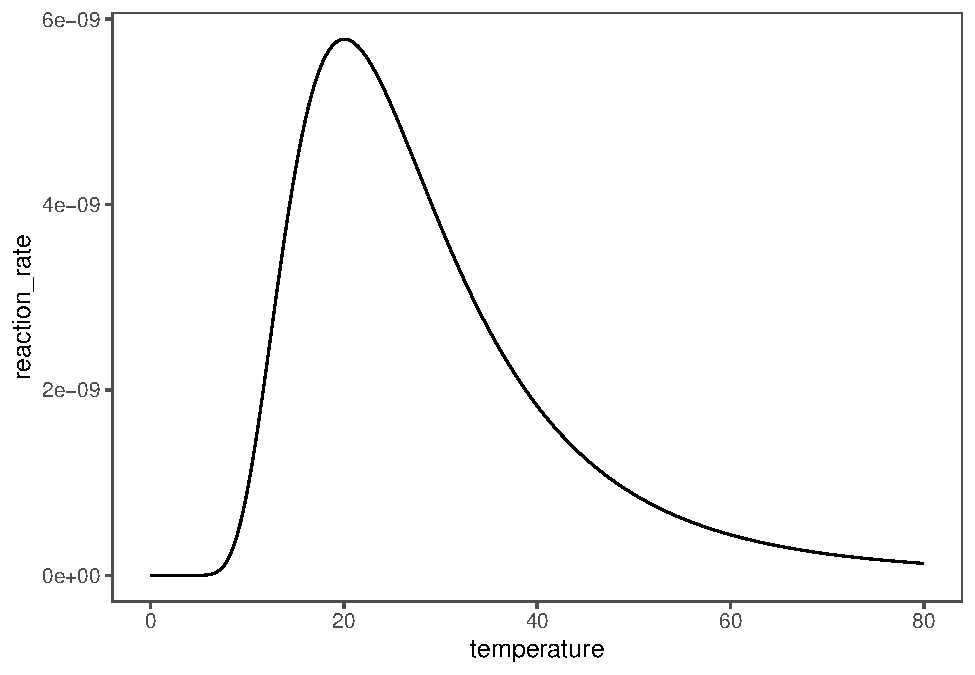
\includegraphics{Bioprocess_Engineering_files/figure-latex/unnamed-chunk-5-1.pdf}

We will describe this behavior mathematically later on, when we derive the rate equation for enzymes.

\hypertarget{fc_i-decreases-as-the-concentrations-of-the-reactants-decrease}{%
\paragraph{\texorpdfstring{\(f(C_i)\) decreases as the concentrations of the reactants decrease}{f(C\_i) decreases as the concentrations of the reactants decrease}}\label{fc_i-decreases-as-the-concentrations-of-the-reactants-decrease}}

For a given temperature the rate of a reaction will decrease as the concentrations of the reactants decrease. This generalization again is true for most elementary reactions, but is violated in many enzymatic (and other catalytic) reactions, where extremely high substrate concentrations can inhibit some enzymes. We will also discuss this behavior while deriving the rate equations for enzymes.

\hypertarget{fc_i-describes-the-order-of-the-reaction-for-each-species}{%
\paragraph{\texorpdfstring{\(f(C_i)\) describes the order of the reaction for each species}{f(C\_i) describes the order of the reaction for each species}}\label{fc_i-describes-the-order-of-the-reaction-for-each-species}}

This generalization dictates that \(f(C_i)\) can be written as the product of all species raised to their ``order'' in the reaction.
\[f(C_i) \approx \prod_{i} C_i^{\alpha_i} \]
where \(\alpha_i\) is the order of the reaction for species \(i\). The order of reaction generally ranges from -2 to 2 (fractional values are permissible). The summation \(\sum_i \alpha_i\) is referred to as the overall order of reaction.

The order of the reaction for a species reflects the sensitivity of the rate of reaction to a change in concentration of species \(i\). If \(\alpha_i = 0\) then the reaction rate is unaffected by the concentration of \(i\). If \(\alpha_i < 0\) then the reaction rate is slowed---or inhibited---by \(i\).

Rate equations which obey this behavior are called power-law rate equations. These equations are grounded in thermodynamics governing molecular collisions between reactants and are often a useful starting point for analysis of kinetic data. Using a power law rate equation to describe the reaction:
\[\ce{(-\nu_{A})A + (-\nu_{B})B -> \nu_{C}C + \nu_{D}D}\]
we would propose that
\[f(C_i) = C_A^{\alpha_A}C_B^{\alpha_B}C_C^{\alpha_C}C_D^{\alpha_D}\]
The reaction orders cannot be determined from the stoichiometry of a reaction, \emph{i.e.} \(\alpha_i \ne -\nu_i\). There are many ways to write a balanced stoichiometric equation for a reaction, the coefficients can be multiplied by any number. The reaction order reflects the actual behavior and mechanism of the reaction. We cannot assume to know which balanced equation reflects the mechanism, but we can hypothesize a mechanism and check if kinetic data fits. We will do this in a later section.

In the case that the reaction orders match the stoichiometry of the reaction as written, this reaction is called \textbf{elementary}. Elementary reactions are critical the development of reaction mechanisms and kinetics. We will discuss elementary reactions more in the next section.

Once again, for enzymatic reactions, this generalization does not hold. We will soon see enzymatic reactions are more representative of multiple reactions. This generalization may hold for the individual reactions comprising the enzymatic mechanism. But for the reaction as a whole, we will soon see, the order of reaction varies with substrate concentration.

\hypertarget{for-reversible-reactions-the-net-rate-is-the-difference-between-the-forward-and-reverse-reactions}{%
\paragraph{For reversible reactions, the net rate is the difference between the forward and reverse reactions}\label{for-reversible-reactions-the-net-rate-is-the-difference-between-the-forward-and-reverse-reactions}}

\[-r_{A,net} = -r_{A,f}-r_{A,r}\]
Here \(-r_{A,net}\) is the total rate at which the reaction proceeds and species A is a reactant as the chemical equation is written. The reaction is moving forward, if \(-r_{A,net}\) is positive, because the rate of consumption of A in the forward reaction, \(-r_{A,f}\), is greater than the rate of formation of A by the reverse reaction, \(r_{A,r}\). Don't forget the convention that rates of reaction are positive and the sign is determined by the stoichiometry of the reaction.

Based on this generalization we can derive the equilibrium expression for a reversible reaction. At equilibrium the net rate of reaction is 0 and we can write out the rates of the forward and reverse reactions according to the order of reaction in each species.
\[0 = -r_{A,f} - r_{A,r} = k_f \prod_i C_i^{\alpha_{f,i}} - k_r \prod_i C_i^{\alpha_{r,i}}\]

Rearranging we define the the equilibrium constant,
\[ K_{eq}^C = \frac{k_f}{k_r} = \prod_i C_i^{(\alpha_{r,i} - \alpha{f,i})}\]

This was derived completely from the principles of kinetics. An equilibrium constant can also be derived via thermodynamics. As you might remember from thermodynamics:
\[K_{eq} = \prod_i a_i^{\nu_i}\]
where \(a_i\) is the activity (or ``effective concentration'') of species \(i\). This expression for the equilibrium constant depends on the way the stoichiometric coefficients and thus the way the chemical equation is written. For a typical aqueous reaction we can write this equation in terms of concentration
\[K_{eq}^C=\prod_iC_i^{\nu_i}\]
Comparing the thermodynamic and kinetic definitions of \(K_{eq}^C\) we can see potential for inconsistency depending on how our chemical equation is written. This implies that in order to be thermodynamically consistent we must define the equilibrium constant based on a single balanced chemical equation. By setting the two versions of the equilibrium constant equal, we can define the condition for this correct equation.
\[\nu_i = \alpha_{r,i} - \alpha_{f,i}\]
Simply, the stoichiometric coefficients must be equal to the order of the total reaction.

\hypertarget{elementary-reactions}{%
\subsection{Elementary reactions}\label{elementary-reactions}}

The above statement defines an elementary reaction, \emph{i.e.} the order of the forward reaction with respect to species \emph{i} is equal to the number of molecules of species \emph{i} participating in each individual reaction. The same is true for the reverse reaction. So for the simple example reaction
\[ \ce{2A <=> B} \]
the rate of the forward reaction is given by \(-r_{A,f} = k_f C_A^2\), and the rate of the reverse reaction \(r_{A,r} = k_r C_B\). Combining the two rate equations we find the net rate of disappearance of A is \(-r_{A,net}=k_f C_A^2 - k_r C_B\). In these equation the rate constants are defined in terms of A so the units of \(k_f\) are (volume/mole A-time) and the units of \(k_r\) are (mole A/mole B-time). Unfortunately, the units first order rate constants are often written just as (time\textsuperscript{-1}).

\hypertarget{questions-2}{%
\paragraph{???Questions???}\label{questions-2}}

How would you write the net rate of formation of B?

\begin{quote}
\emph{Using stoichiometry, \(r_B = \frac{1}{2}(-r_A)\). Similarly the rate constants can be rewritten in terms of B.}
\end{quote}

\begin{center}\rule{0.5\linewidth}{0.5pt}\end{center}

\hypertarget{properties-of-elementary-reactions}{%
\subsubsection{Properties of Elementary Reactions}\label{properties-of-elementary-reactions}}

What assumptions can we make to help us propose elementary reactions?

\begin{enumerate}
\def\labelenumi{\arabic{enumi}.}
\item
  An elementary reaction---a single-step, molecular level event---must be simple. It likely only involves two molecules, as termolecular collisions are very unlikely, and such collisions happening in the correct orientation are even less likely. We can also assume very few bonds will be formed or broken in a single step.
\item
  Elementary reactions cannot involve fractional molecules.
\item
  Elementary reactions must obey the principle of microscopic reversibility. Microscopic reversibility means that the reaction must follow the same mechanism in the forward and reverse directions. This means that an elementary reaction must be elementary in both directions.
\end{enumerate}

With this framework for writing elementary reactions we will in Chapter 4 begin deriving mechanisms and rate equations for more complex reactions, which are actually series of multiple elementary reactions.

For now we will assume all of the reactions we are dealing with are elementary, unless we are given a rate equation, and we will begin to examine the kinetics of reactions in ideal reactors.

\hypertarget{ideal-reactors}{%
\section{Ideal Reactors}\label{ideal-reactors}}

Before jumping into more complex kinetics we will first discuss chemical reactors for simple, elementary reactions. This will give us an understanding of what different reaction orders mean and how reversibility affects dynamics. We will also gain and understanding of different chemical reactors and how reactor choice can effect the reaction outcome.

For any reactor we can consider a small control volume \(dV\), and examine the rate of generation of species \(i\) in that control volume:
\[G_i = \iiint_V r_idV\]
For open systems, e.g.~continuous flow reactors we will have some flow rate into and out of this volume element. Remembering your basic material balances:
\[\text{Rate In - Rate Out + Rate of Generation = Rate of Accumulation}\]
\[F_{i0} - F_i + G_i = \frac{dN_i}{dt}\]
Now let's consider three types of ideal reactors that this generalized control volume could be in.

\hypertarget{batch-reactors}{%
\subsection{Batch Reactors}\label{batch-reactors}}

In most cases, examination of a chemical or biochemical reaction will begin with a small scale batch reactor. An ideal batch reactor is defined as a fixed volume, with no flow in or out, that is well mixed such that concentration and temperature are uniform throughout the volume. The concentration and temperature can vary overtime as the reaction proceeds, but typically some temperature-control mechanism will be applied such that the reactor can be considered isothermal.

For batch reactors \(F_{i0} = F_i = 0\), such that the rate of generation of species \(i\) becomes:
\[G_i = \iiint_V r_idV = \frac{dN_i}{dt}\]
Since perfect mixing renders \(r_i\) independent of position integration is simple yielding
\[r_i =\frac{1}{V} \frac{dN_i}{dt}\]
This equation is called the \textbf{design equation} for a batch reactor.
We can substitute \(r_i\) for the overall rate equation for any reaction or multiple reactions, and if we can separate the variables dependent on species \(i\) and time, we can solve this equation to yield an expression for the number of moles of species \(i\) versus time.

We can also write this design equation in terms of extent of reaction, as extent of reaction, \(\xi = \Delta N_i / \nu_i\).
\[r_i = \frac{\nu_i}{V} \frac{d\xi}{dt}\]
Additionally for single reactions it is sometimes useful to write the design equation in terms of the fraction of the limiting reactant, \(l\) that has been consumed, or fractional conversion, \(x_l\).

In this case the design equation is
\[-r_l = \frac{N_{l0}}{V} \frac{dx_l}{dt}\]
If volume is constant, we can also write any of these equations in terms of concentration as \(C_i = N_i / V\), \emph{e.g.}
\[r_i =\frac{dC_i}{dt}\]
If there is a catalyst or enzyme in the reactor we can also replace the volume of the reactor with the mass of the catalyst in the reactor in any of these equations.

Solving these differential equations will provide us with an equation for the amount of species \(i\) in the reactor at any given time during the reaction. This will then allow us to calculate the amount of time or reactor volume necessary to run a reaction to achieve the desired quantity of product.

Let's do some example calculations.

\hypertarget{first-order-reaction-example}{%
\subsubsection{First Order Reaction Example}\label{first-order-reaction-example}}

Consider a liquid phase reaction \(\ce{A -> B}\) that is elementary, therefore the rate equation can be written as \(-r_A = r_B = k_1C_A\). How long must the reactor be run in order for 70\% of A to be converted to B if \(k_1 = 0.05 \text{ min}^{-1}\) and \(C_{A0} = 5 \text{ M}\)?

Our goal is to find the time required for 70\% of A to be consumed. This indicates that we should set this problem up in terms of fractional conversion or extent of reaction. So our design equation will simplify to
\[r_A = \frac{dC_A}{dt} = \frac{d[C_{A0}(1-x_A)]}{dt} = \frac{d(C_{A0}-C_{A0}x_A)}{dt} = 0-C_{A0}\frac{dx_A}{dt}\]
\[-r_A = C_{A0}\frac{dX_A}{dt}\]

We know what the rate of consumption of A is since the reaction is elementary, so we can plug this relation in for \(-r_A\), and also write \(C_A\) in terms of fractional conversion, \(C_{A0}(1-x_A)\).
\[k_1C_{A0}(1-x_A) =  C_{A0} \frac{dx_A}{dt}\]
We can then separate variables
\[k_1dt = \frac{dx_A}{(1-x_A)}\]
and finally integrate
\[k_1\int_0^tdt = \int_0^{0.7}\frac{1}{(1-x_A)} dx_A\]
to yield
\[t = \frac{-[\ln(1-0.7)-\ln(1)]}{k_1}\]

So in this case 24.08 minutes are required to achieve 70\% conversion.

What do the dynamics of this reaction look like over time? Let's solve the general form of the integral to find out.
\[k_1\int_0^tdt = \int_0^{x_A}\frac{1}{(1-x_A)} dx_A\]
\[t = \frac{-\ln(1-x_A)}{k_1} \]
\[e^{-k_1t} = 1-x_A\]
\[x_A = 1-e^{-k_1t}\]
Now we can plot this relationship.

\begin{Shaded}
\begin{Highlighting}[]
\NormalTok{k\_1 }\OtherTok{\textless{}{-}} \FloatTok{0.05}
\NormalTok{t }\OtherTok{\textless{}{-}} \FunctionTok{seq}\NormalTok{(}\DecValTok{0}\NormalTok{, }\DecValTok{100}\NormalTok{, }\FloatTok{0.1}\NormalTok{)}
\NormalTok{x\_A }\OtherTok{\textless{}{-}} \DecValTok{1} \SpecialCharTok{{-}} \FunctionTok{exp}\NormalTok{(}\SpecialCharTok{{-}}\NormalTok{k\_1 }\SpecialCharTok{*}\NormalTok{ t)}
\FunctionTok{require}\NormalTok{(tidyverse)}
\FunctionTok{require}\NormalTok{(magrittr)}
\NormalTok{data }\OtherTok{\textless{}{-}} \FunctionTok{tibble}\NormalTok{(t, x\_A)}
\FunctionTok{ggplot}\NormalTok{(}\AttributeTok{data =}\NormalTok{ data, }\FunctionTok{aes}\NormalTok{(}\AttributeTok{x =}\NormalTok{ t, }\AttributeTok{y =}\NormalTok{ x\_A)) }\SpecialCharTok{+} \FunctionTok{geom\_line}\NormalTok{() }\SpecialCharTok{+}
    \FunctionTok{coord\_cartesian}\NormalTok{(}\AttributeTok{ylim =} \FunctionTok{c}\NormalTok{(}\DecValTok{0}\NormalTok{, }\DecValTok{1}\NormalTok{))}
\end{Highlighting}
\end{Shaded}

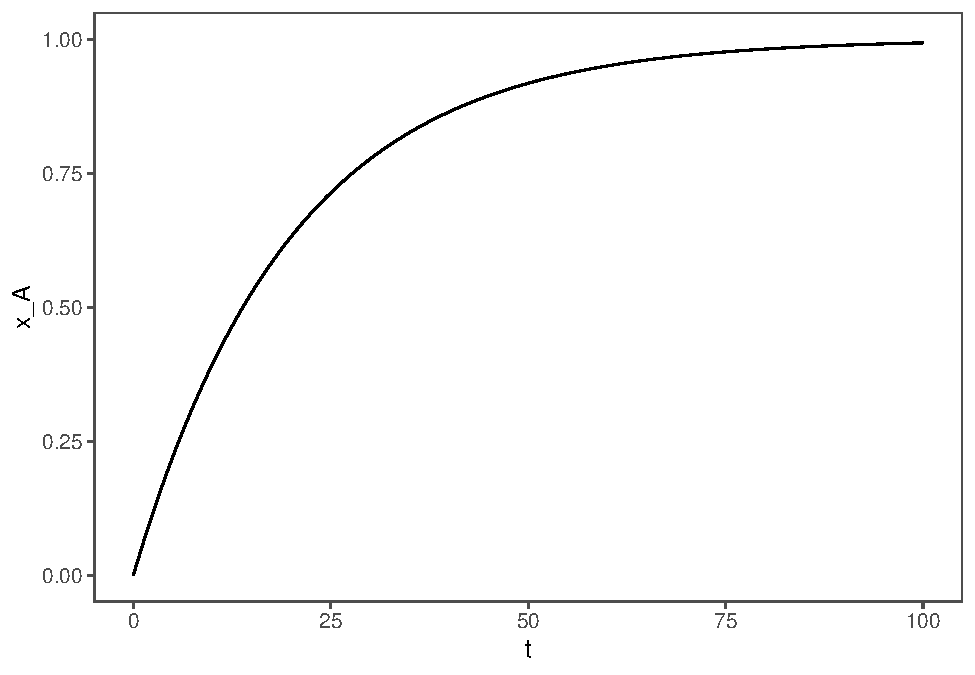
\includegraphics{Bioprocess_Engineering_files/figure-latex/unnamed-chunk-8-1.pdf}

As we calculated we would need to run the reaction for \textasciitilde24 minutes to achieve 70\% conversion.

\hypertarget{questions-3}{%
\paragraph{???Questions???}\label{questions-3}}

Does the reaction ever reach 100\% conversion?

\begin{quote}
\emph{No, it asymptotically approaches it.}
\end{quote}

\begin{center}\rule{0.5\linewidth}{0.5pt}\end{center}

What do the concentrations of A and B look like over time?

For this let's make a stoichiometric table to help us keep everything straight

\begin{longtable}[]{@{}ccc@{}}
\toprule\noalign{}
Species & Initial Concentration & Concentration at t=t \\
\midrule\noalign{}
\endhead
\bottomrule\noalign{}
\endlastfoot
A & \(C_{A0}\) & \(C_{A0}(1-x_A)\) \\
B & \(0\) & \(C_{A0}x_A\) \\
\end{longtable}

Now we can add these concentrations to our plot.

\begin{Shaded}
\begin{Highlighting}[]
\NormalTok{C\_A0 }\OtherTok{\textless{}{-}} \DecValTok{5}  \CommentTok{\#M}
\NormalTok{C\_A }\OtherTok{\textless{}{-}}\NormalTok{ C\_A0 }\SpecialCharTok{*}\NormalTok{ (}\DecValTok{1} \SpecialCharTok{{-}}\NormalTok{ data}\SpecialCharTok{$}\NormalTok{x\_A)}
\NormalTok{C\_B }\OtherTok{\textless{}{-}}\NormalTok{ C\_A0 }\SpecialCharTok{*}\NormalTok{ data}\SpecialCharTok{$}\NormalTok{x\_A}
\NormalTok{data }\OtherTok{\textless{}{-}} \FunctionTok{cbind}\NormalTok{(data, C\_A, C\_B)}
\CommentTok{\# we could also use a \textquotesingle{}pipe\textquotesingle{} to send data as the}
\CommentTok{\# first argument data \%\textless{}\textgreater{}\% cbind(C\_A, C\_B) We}
\CommentTok{\# need to tidy this data up a bit Gather the}
\CommentTok{\# Concentration values into a single column and}
\CommentTok{\# create a new key column Species}

\NormalTok{data }\SpecialCharTok{\%\textless{}\textgreater{}\%}
    \FunctionTok{gather}\NormalTok{(C\_A, C\_B, }\AttributeTok{key =} \StringTok{"Species"}\NormalTok{, }\AttributeTok{value =} \StringTok{"Concentration"}\NormalTok{)}
\FunctionTok{ggplot}\NormalTok{(}\AttributeTok{data =}\NormalTok{ data, }\FunctionTok{aes}\NormalTok{(}\AttributeTok{x =}\NormalTok{ t, }\AttributeTok{y =}\NormalTok{ Concentration, }\AttributeTok{color =}\NormalTok{ Species)) }\SpecialCharTok{+}
    \FunctionTok{geom\_line}\NormalTok{()}
\end{Highlighting}
\end{Shaded}

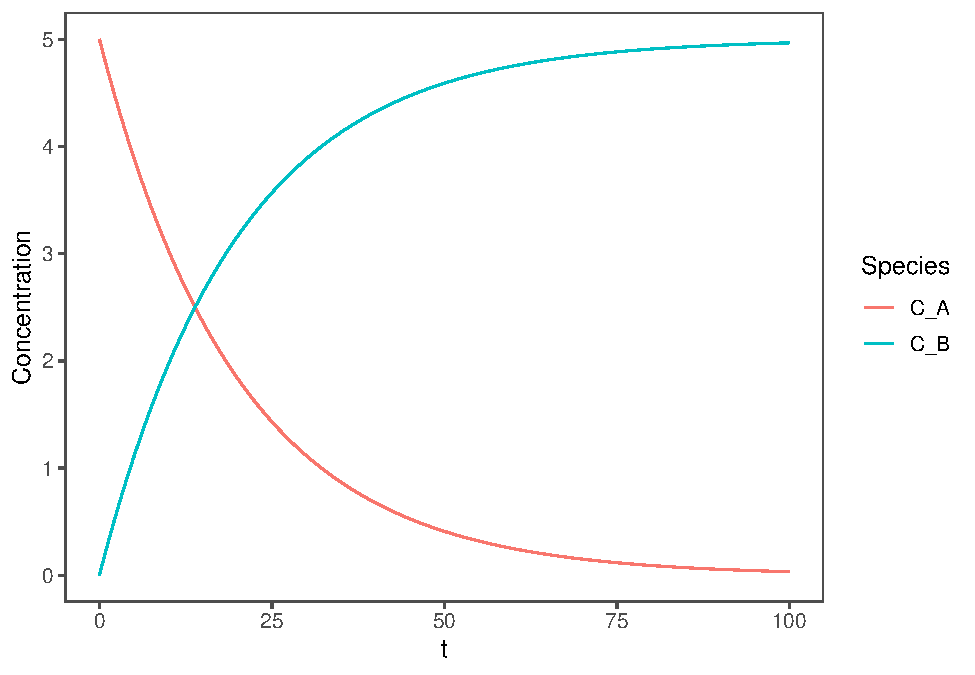
\includegraphics{Bioprocess_Engineering_files/figure-latex/unnamed-chunk-10-1.pdf}

\hypertarget{questions-4}{%
\paragraph{???Questions???}\label{questions-4}}

What would the above plot look like if the reaction were zero order? \emph{E.g.} if the reaction was \(\ce{ A -> B }\) and the rate equation was \(-r_A = k_1\)

\begin{quote}
\emph{The design equation for a zero order batch reaction simplifies to \(k_1 = C_{A0} \frac{dx_A}{dt}\). Integrating this yields \(x_A = k_1t\). Graphing this equation as above yields }
\end{quote}

\begin{Shaded}
\begin{Highlighting}[]
\NormalTok{x\_A }\OtherTok{\textless{}{-}}\NormalTok{ k\_1 }\SpecialCharTok{*}\NormalTok{ t}
\FunctionTok{require}\NormalTok{(tidyverse)}
\FunctionTok{require}\NormalTok{(magrittr)}
\NormalTok{data }\OtherTok{\textless{}{-}} \FunctionTok{tibble}\NormalTok{(t, x\_A)}
\NormalTok{C\_A }\OtherTok{\textless{}{-}}\NormalTok{ C\_A0 }\SpecialCharTok{*}\NormalTok{ (}\DecValTok{1} \SpecialCharTok{{-}}\NormalTok{ data}\SpecialCharTok{$}\NormalTok{x\_A)}
\NormalTok{C\_B }\OtherTok{\textless{}{-}}\NormalTok{ C\_A0 }\SpecialCharTok{*}\NormalTok{ data}\SpecialCharTok{$}\NormalTok{x\_A}
\NormalTok{data }\OtherTok{\textless{}{-}} \FunctionTok{cbind}\NormalTok{(data, C\_A, C\_B)}
\NormalTok{data }\SpecialCharTok{\%\textless{}\textgreater{}\%}
    \FunctionTok{gather}\NormalTok{(C\_A, C\_B, }\AttributeTok{key =} \StringTok{"Species"}\NormalTok{, }\AttributeTok{value =} \StringTok{"Concentration"}\NormalTok{)}
\FunctionTok{ggplot}\NormalTok{(}\AttributeTok{data =}\NormalTok{ data, }\FunctionTok{aes}\NormalTok{(}\AttributeTok{x =}\NormalTok{ t, }\AttributeTok{y =}\NormalTok{ Concentration, }\AttributeTok{color =}\NormalTok{ Species)) }\SpecialCharTok{+}
    \FunctionTok{geom\_line}\NormalTok{() }\SpecialCharTok{+} \FunctionTok{coord\_cartesian}\NormalTok{(}\AttributeTok{ylim =} \FunctionTok{c}\NormalTok{(}\DecValTok{0}\NormalTok{, }\DecValTok{5}\NormalTok{), }\AttributeTok{xlim =} \FunctionTok{c}\NormalTok{(}\DecValTok{0}\NormalTok{,}
    \DecValTok{20}\NormalTok{))}
\end{Highlighting}
\end{Shaded}

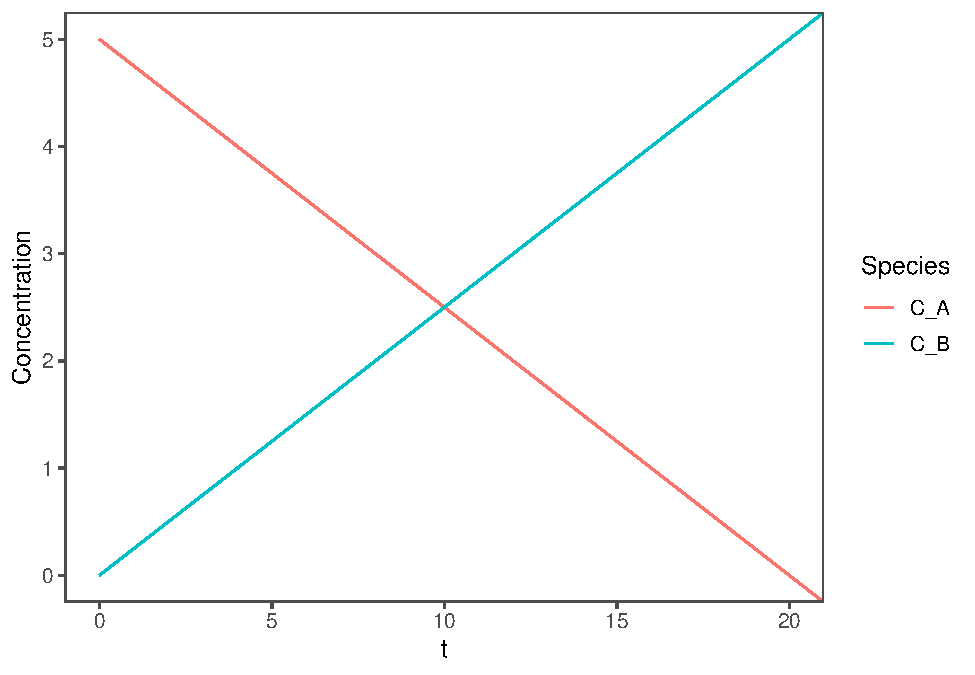
\includegraphics{Bioprocess_Engineering_files/figure-latex/zero-order-1.pdf}

\begin{quote}
\emph{This plot is only valid for the window of time for which \(C_A\) is positive, as concentrations cannot be negative. To truly represent zero order reactions across indefinite times a discontinuous function must be used.}
\end{quote}

\begin{center}\rule{0.5\linewidth}{0.5pt}\end{center}

\hypertarget{second-order-reaction-example}{%
\subsubsection{Second-order Reaction Example}\label{second-order-reaction-example}}

\hypertarget{questions-5}{%
\paragraph{???Questions???}\label{questions-5}}

What would this plot look like if it were second order?
\emph{E.g.} if the reaction was \(\ce{ 2A -> B }\) and the rate equation was \(-r_A = k_1C_A^2\)

\begin{quote}
\[-r_A = C_{A0}\frac{dX_A}{dt}\]
\emph{In this case the design equation simplifies to}
\[k_1C_{A0}(1-x_A)^2 = \frac{dx_A}{dt}\]
\[\int_0^tk_1C_{A0}dt = \int_0^{x_A}\frac{dx_A}{(1-x_A)^2}\]
\[k_1C_{A0}t = \frac{1}{1-x_A} - 1\]
\[ 1 - x_A = \frac{1}{k_1C_{A0}t + 1}\]
\[ x_A = 1 - \frac{1}{k_1C_{A0}t + 1}\]
\emph{Graphing this equation as above yields}
\end{quote}

\begin{Shaded}
\begin{Highlighting}[]
\NormalTok{x\_A }\OtherTok{\textless{}{-}} \DecValTok{1} \SpecialCharTok{{-}} \DecValTok{1}\SpecialCharTok{/}\NormalTok{(k\_1 }\SpecialCharTok{*}\NormalTok{ C\_A0 }\SpecialCharTok{*}\NormalTok{ t }\SpecialCharTok{+} \DecValTok{1}\NormalTok{)}
\FunctionTok{require}\NormalTok{(tidyverse)}
\FunctionTok{require}\NormalTok{(magrittr)}
\NormalTok{data }\OtherTok{\textless{}{-}} \FunctionTok{tibble}\NormalTok{(t, x\_A)}
\NormalTok{C\_A }\OtherTok{\textless{}{-}}\NormalTok{ C\_A0 }\SpecialCharTok{*}\NormalTok{ (}\DecValTok{1} \SpecialCharTok{{-}}\NormalTok{ data}\SpecialCharTok{$}\NormalTok{x\_A)}
\NormalTok{C\_B }\OtherTok{\textless{}{-}}\NormalTok{ C\_A0 }\SpecialCharTok{*}\NormalTok{ data}\SpecialCharTok{$}\NormalTok{x\_A}\SpecialCharTok{/}\DecValTok{2}
\NormalTok{data }\OtherTok{\textless{}{-}} \FunctionTok{cbind}\NormalTok{(data, C\_A, C\_B)}
\NormalTok{data }\SpecialCharTok{\%\textless{}\textgreater{}\%}
    \FunctionTok{gather}\NormalTok{(C\_A, C\_B, }\AttributeTok{key =} \StringTok{"Species"}\NormalTok{, }\AttributeTok{value =} \StringTok{"Concentration"}\NormalTok{)}
\FunctionTok{ggplot}\NormalTok{(}\AttributeTok{data =}\NormalTok{ data, }\FunctionTok{aes}\NormalTok{(}\AttributeTok{x =}\NormalTok{ t, }\AttributeTok{y =}\NormalTok{ Concentration, }\AttributeTok{color =}\NormalTok{ Species)) }\SpecialCharTok{+}
    \FunctionTok{geom\_line}\NormalTok{()}
\end{Highlighting}
\end{Shaded}

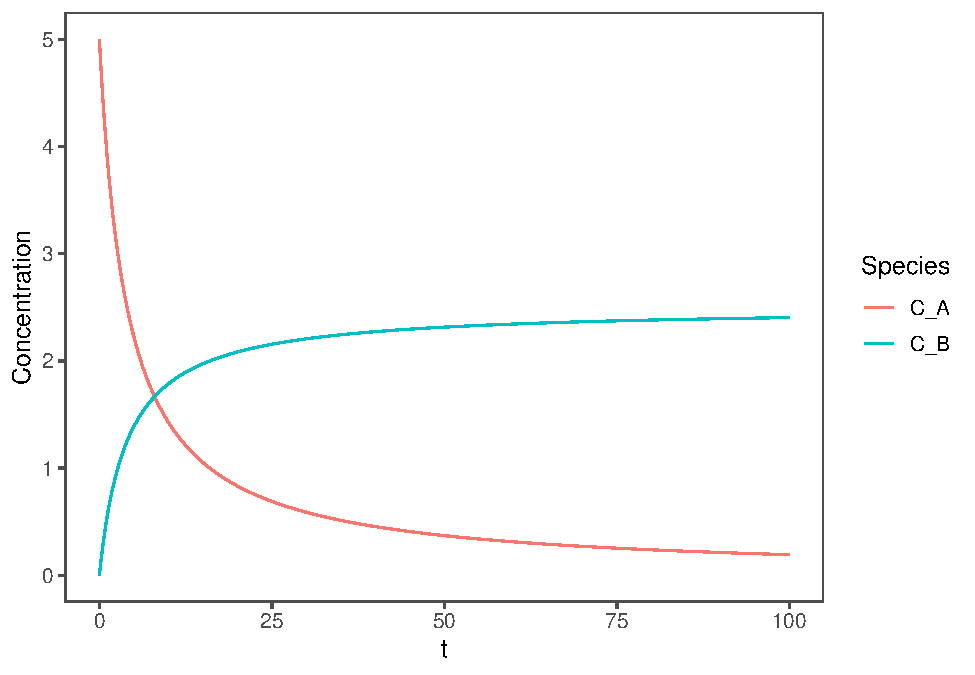
\includegraphics{Bioprocess_Engineering_files/figure-latex/second-order-1.pdf}

\begin{center}\rule{0.5\linewidth}{0.5pt}\end{center}

\hypertarget{reversible-first-order-reaction-example}{%
\subsubsection{Reversible first-order reaction example}\label{reversible-first-order-reaction-example}}

What about if this were first-order and reversible?
\[\ce{ A <=> B }\]
\[-r_A = k_fC_A - k_rC_B\]
Because reversible reactions are actually multiple reactions we cannot use fractional conversion or extent of reaction to measure this reaction, we will just use concentrations.

Let's make a stoichiometric table to start in terms of reactant A.

\begin{longtable}[]{@{}ccc@{}}
\toprule\noalign{}
Species & Initial Concentration & Concentration at t=t \\
\midrule\noalign{}
\endhead
\bottomrule\noalign{}
\endlastfoot
A & \(C_{A0}\) & \(C_A\) \\
B & \(0\) & \(C_{A0}-C_A\) \\
\end{longtable}

Now we can rewrite the rate equation based on this table.
\[-r_A = k_fC_A - k_r(C_{A0}-C_A)\]
And so the design equation (material balance) is
\[\frac{dC_A}{dt} = k_fC_A - k_r(C_{A0}-C_A)\]
\[\int_0^{C_A}\frac{dC_A}{(k_f + k_r)C_A - k_rC_{A0}} = \int_0^tdt \]
Integrating and solving for \(C_A\) we get:
\[C_A = \frac{k_fC_{A0}e^{-(k_f+k_r)t} + C_{A0}k_r}{k_f+k_r}\]
Now we can plot this assuming the same conditions (\(k_f = 0.05\text{ min}^{-1}\) and \(C_{A0} = 5\text{ M}\)) as above, and we can vary the ratio of \(k_f/k_r\).

\begin{Shaded}
\begin{Highlighting}[]
\NormalTok{C\_A0 }\OtherTok{\textless{}{-}} \DecValTok{5}  \CommentTok{\#M}
\NormalTok{k\_f }\OtherTok{\textless{}{-}} \FloatTok{0.05}  \CommentTok{\#min}
\NormalTok{kf\_kr }\OtherTok{\textless{}{-}} \FunctionTok{c}\NormalTok{(}\DecValTok{10}\NormalTok{, }\DecValTok{1}\NormalTok{, }\FloatTok{0.1}\NormalTok{)}
\NormalTok{k\_r }\OtherTok{\textless{}{-}}\NormalTok{ k\_f}\SpecialCharTok{/}\NormalTok{kf\_kr}
\FunctionTok{require}\NormalTok{(tidyverse)}
\FunctionTok{require}\NormalTok{(magrittr)}
\CommentTok{\# now we are going to need to apply our C\_A}
\CommentTok{\# calculation over each of the k\_r values to do}
\CommentTok{\# this we will make C\_A a function}
\NormalTok{C\_A }\OtherTok{\textless{}{-}} \ControlFlowTok{function}\NormalTok{(k\_f, C\_A0, k\_r, t) \{}
\NormalTok{    (k\_f }\SpecialCharTok{*}\NormalTok{ C\_A0 }\SpecialCharTok{*} \FunctionTok{exp}\NormalTok{(}\SpecialCharTok{{-}}\NormalTok{(k\_f }\SpecialCharTok{+}\NormalTok{ k\_r) }\SpecialCharTok{*}\NormalTok{ t) }\SpecialCharTok{+}\NormalTok{ C\_A0 }\SpecialCharTok{*}\NormalTok{ k\_r)}\SpecialCharTok{/}\NormalTok{(k\_f }\SpecialCharTok{+}
\NormalTok{        k\_r)}
\NormalTok{\}}
\CommentTok{\# and make a table of all combinations of times}
\CommentTok{\# and k\_r\textquotesingle{}s}
\NormalTok{data }\OtherTok{\textless{}{-}} \FunctionTok{crossing}\NormalTok{(k\_r, t)}
\NormalTok{data }\SpecialCharTok{\%\textless{}\textgreater{}\%}
    \FunctionTok{add\_column}\NormalTok{(k\_f, C\_A0, }\AttributeTok{.before =} \ConstantTok{TRUE}\NormalTok{)}
\CommentTok{\# now apply this function over all values of k\_r}
\CommentTok{\# and t}
\NormalTok{data }\SpecialCharTok{\%\textless{}\textgreater{}\%}
    \FunctionTok{mutate}\NormalTok{(}\AttributeTok{C\_A =} \FunctionTok{unlist}\NormalTok{(}\FunctionTok{pmap}\NormalTok{(., C\_A)))}
\NormalTok{data}\SpecialCharTok{$}\NormalTok{C\_B }\OtherTok{\textless{}{-}}\NormalTok{ C\_A0 }\SpecialCharTok{{-}}\NormalTok{ data}\SpecialCharTok{$}\NormalTok{C\_A}
\NormalTok{data }\SpecialCharTok{\%\textless{}\textgreater{}\%}
    \FunctionTok{gather}\NormalTok{(C\_A, C\_B, }\AttributeTok{key =} \StringTok{"Species"}\NormalTok{, }\AttributeTok{value =} \StringTok{"Concentration"}\NormalTok{)}
\NormalTok{data}\SpecialCharTok{$}\NormalTok{kf\_kr }\OtherTok{\textless{}{-}}\NormalTok{ data}\SpecialCharTok{$}\NormalTok{k\_f}\SpecialCharTok{/}\NormalTok{data}\SpecialCharTok{$}\NormalTok{k\_r}
\FunctionTok{ggplot}\NormalTok{(}\AttributeTok{data =}\NormalTok{ data, }\FunctionTok{aes}\NormalTok{(}\AttributeTok{x =}\NormalTok{ t, }\AttributeTok{y =}\NormalTok{ Concentration, }\AttributeTok{color =}\NormalTok{ Species,}
    \AttributeTok{linetype =} \FunctionTok{as.factor}\NormalTok{(kf\_kr))) }\SpecialCharTok{+} \FunctionTok{geom\_line}\NormalTok{()}
\end{Highlighting}
\end{Shaded}

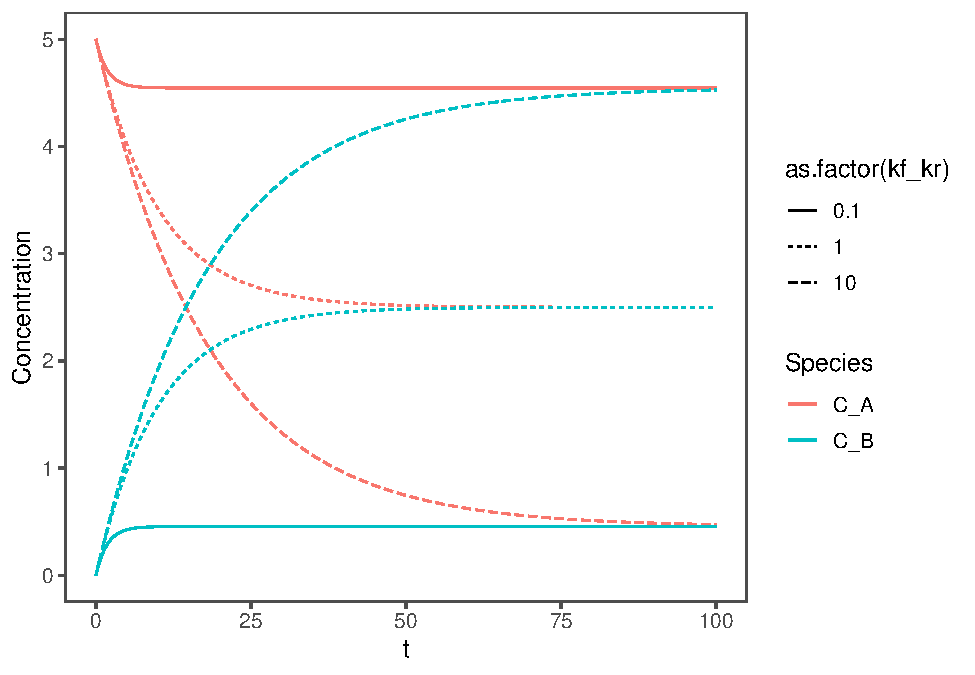
\includegraphics{Bioprocess_Engineering_files/figure-latex/unnamed-chunk-14-1.pdf}

\hypertarget{continuous-stirred-tank-reactors}{%
\subsection{Continuous-stirred tank reactors}\label{continuous-stirred-tank-reactors}}

Continuous-stirred tank reactors, or CSTRs, are just like batch reactors except with continuous feed and effluent streams. Ideal mixing is still in effect equalizing temperature and concentration across the contents of the reactor. So to adapt the general equations for a CSTR we simply keep all terms:
\[F_{i0} - F_i + r_iV = \frac{dN_i}{dt}\]
If assumptions such as constant volume or a single reaction are valid we can similarly simplify this equation to be in terms of concentrations or fractional conversion and extent of reaction, respectively. It is always best to start with the general design equation and walk through each assumption to simplify it, instead of jumping straight to a simplified version without fully assessing each assumption.

For CSTRs the rates of reaction are defined at the effluent conditions, which because of perfect mixing are equivalent to the reaction conditions in the entire reactor.

For continuous flow reactors we need to define a quantity that reflects how long the reactants spend in the reactor. Most often a quantity called \textbf{space time} is used. Space time is related to the average time that any unit fluid spends in the reactor. Space time at inlet conditions is defined as
\[\tau_0 = V/v_0\]
where \(v_0\) is the inlet volumetric flowrate.

Space time provides an analagous metric to real time in a batch reactor. If a batch reaction is run for a longer time more reactants will be converted to product, and if a continuous reactor is run at higher space time, more reactants will be converted to product in the effluent.

As \(F_{i0} = C_{i0}v_0\), for constant volume reactions, that is when fluid density is constant throughout the reaction, the design equation can be written in terms of space time
\[\tau_0 = \frac{C_{i0}x_i}{r_i}\]
Also analagous to batch reactors, catalyst or enzyme weight can also be swapped for reactor volume in the CSTR design equations and definitions of space time. In these cases the catalysts or enzymes are often immobilized on polymeric beads that can easily be filtered from the effluent stream.

\hypertarget{plug-flow-reactors}{%
\subsection{Plug-flow reactors}\label{plug-flow-reactors}}

Alternatively enzyme loaded beads could be packed into a porous bed and reactants could be flowed through this bed. This type of reactor is called a plug-flow reactor. However there does not have to be a packed bed in the reactor at all, you can imagine a pipe with fluid flowing through it and a reaction occuring in that fluid. The further along the length of the pipe the fluid is, the further along the reaction is within that fluid. You might have intuited from that last statement that unlike in batch and continuous stirred tank reactors, in plug-flow reactors the reaction rate varies with position

In order to be an ideal plug flow reactor, two assumptions must be met.
1. There is no mixing in the direction of flow. We can imagine this as little discs or ``plugs'' of fluid moving through the reactor in a single file line, like miniature batch reactors moving through the reactor.
2. There is no variation in temperature or concentration normal to the direction of flow. \emph{I.e.} each of the plugs is uniform.

For a real reactor to approximate an ideal reactor, the flow must be highly turbulent.

For a plug flow reactor (PFR) our material balance simplifies to
\[F_{i0} - F_i + \iiint_V r_i dV = 0\]
As we said before \(r_i\) varies along the length of the reactor and therefore we need to come up with a strategy to solve this integral.

One strategy is to choose a control volume \(dV\) such that \(r_i\) does not vary within \(dV\). So according to our definition of an ideal plug-flow reactor, each ``plug'' would be a perfect control volume becasue the concentration and therefore rate of reaction are uniform across this volume perpendicular to flow. Rewriting our material balance across this control volume:
\[F_i - (F_i + dF_i) + r_i dV = 0\]
So our design equation for a PFR is
\[dV = \frac{dF_i}{r_i}\]

Just as with CSTRs, we can define PFRs in terms of space time and concentration.
\[d\tau_0 = C_{A0} \frac{dx_A}{-r_A}\]

\hypertarget{desigining-continuous-flow-reactors}{%
\subsection{Desigining continuous flow reactors}\label{desigining-continuous-flow-reactors}}

When designing continuous chemical and biochemical reactors we are concerned with the volume of the reactor and flow rate required to meet our production goals. Frequently, a visual representation of the reaction is used to aid in these design decisions for continuous reactors. To derive this visual representation we examine the design equations for a CSTR and PFR.
\[\text{CSTR:   }  \frac{V}{F_{A0}} = \frac{x_{A}}{-r_A} \]
\[\text{PFR:   }  \frac{V}{F_{A0}} = \int_0^{x_A}\frac{dx_{A}}{-r_A} \]
Now if we plot \(1/(-r_A)\) vs \(x_A\), the ratio of the reactor volume to the flow rate for a CSTR is the rectangle where the desired fractional conversion intersects the reaction rate. For a first-order, constant volume, isothermal reaction, this looks like the following:

\begin{Shaded}
\begin{Highlighting}[]
\NormalTok{k\_1 }\OtherTok{\textless{}{-}} \FloatTok{0.05}
\NormalTok{C\_A0 }\OtherTok{\textless{}{-}} \DecValTok{5}  \CommentTok{\#M}
\NormalTok{t }\OtherTok{\textless{}{-}} \FunctionTok{seq}\NormalTok{(}\DecValTok{0}\NormalTok{, }\DecValTok{100}\NormalTok{, }\FloatTok{0.1}\NormalTok{)}
\NormalTok{x\_A }\OtherTok{\textless{}{-}} \DecValTok{1} \SpecialCharTok{{-}} \FunctionTok{exp}\NormalTok{(}\SpecialCharTok{{-}}\NormalTok{k\_1 }\SpecialCharTok{*}\NormalTok{ t)}
\FunctionTok{require}\NormalTok{(tidyverse)}
\FunctionTok{require}\NormalTok{(magrittr)}
\NormalTok{data }\OtherTok{\textless{}{-}} \FunctionTok{tibble}\NormalTok{(t, x\_A)}
\NormalTok{data}\SpecialCharTok{$}\NormalTok{nr\_A }\OtherTok{\textless{}{-}}\NormalTok{ k\_1 }\SpecialCharTok{*}\NormalTok{ (C\_A0) }\SpecialCharTok{*}\NormalTok{ (}\DecValTok{1} \SpecialCharTok{{-}}\NormalTok{ data}\SpecialCharTok{$}\NormalTok{x\_A)}
\FunctionTok{ggplot}\NormalTok{(}\AttributeTok{data =}\NormalTok{ data, }\FunctionTok{aes}\NormalTok{(}\AttributeTok{x =}\NormalTok{ x\_A, }\AttributeTok{y =} \DecValTok{1}\SpecialCharTok{/}\NormalTok{nr\_A)) }\SpecialCharTok{+} \FunctionTok{geom\_line}\NormalTok{() }\SpecialCharTok{+}
    \FunctionTok{annotate}\NormalTok{(}\AttributeTok{geom =} \StringTok{"rect"}\NormalTok{, }\AttributeTok{xmin =} \DecValTok{0}\NormalTok{, }\AttributeTok{xmax =} \FloatTok{0.9}\NormalTok{, }\AttributeTok{ymin =} \DecValTok{0}\NormalTok{,}
        \AttributeTok{ymax =} \DecValTok{1}\SpecialCharTok{/}\NormalTok{data}\SpecialCharTok{$}\NormalTok{nr\_A[}\FunctionTok{min}\NormalTok{(}\FunctionTok{which}\NormalTok{(}\FunctionTok{round}\NormalTok{(data}\SpecialCharTok{$}\NormalTok{x\_A,}
            \DecValTok{3}\NormalTok{) }\SpecialCharTok{==} \FloatTok{0.9}\NormalTok{))], }\AttributeTok{alpha =} \FloatTok{0.5}\NormalTok{)}
\end{Highlighting}
\end{Shaded}

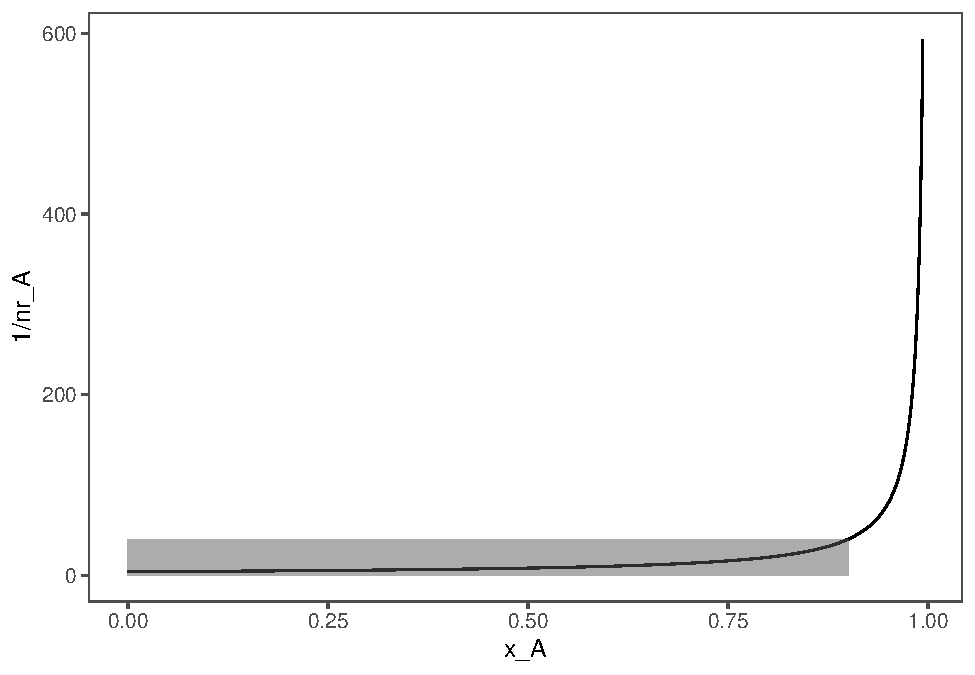
\includegraphics{Bioprocess_Engineering_files/figure-latex/unnamed-chunk-15-1.pdf}

The shaded area in this plot represents the size, \(V\) to flow rate \(F_{A0}\) ratio of the CSTR required to achieve 90\% conversion.
For reference, because thinking in terms of the inverse of the rate is tricky, here is what a plot of the rate equation looks like, \(-r_A\) vs.~\(x_A\):

\begin{Shaded}
\begin{Highlighting}[]
\FunctionTok{ggplot}\NormalTok{(}\AttributeTok{data =}\NormalTok{ data, }\FunctionTok{aes}\NormalTok{(}\AttributeTok{x =}\NormalTok{ x\_A, }\AttributeTok{y =}\NormalTok{ nr\_A)) }\SpecialCharTok{+} \FunctionTok{geom\_line}\NormalTok{()}
\end{Highlighting}
\end{Shaded}

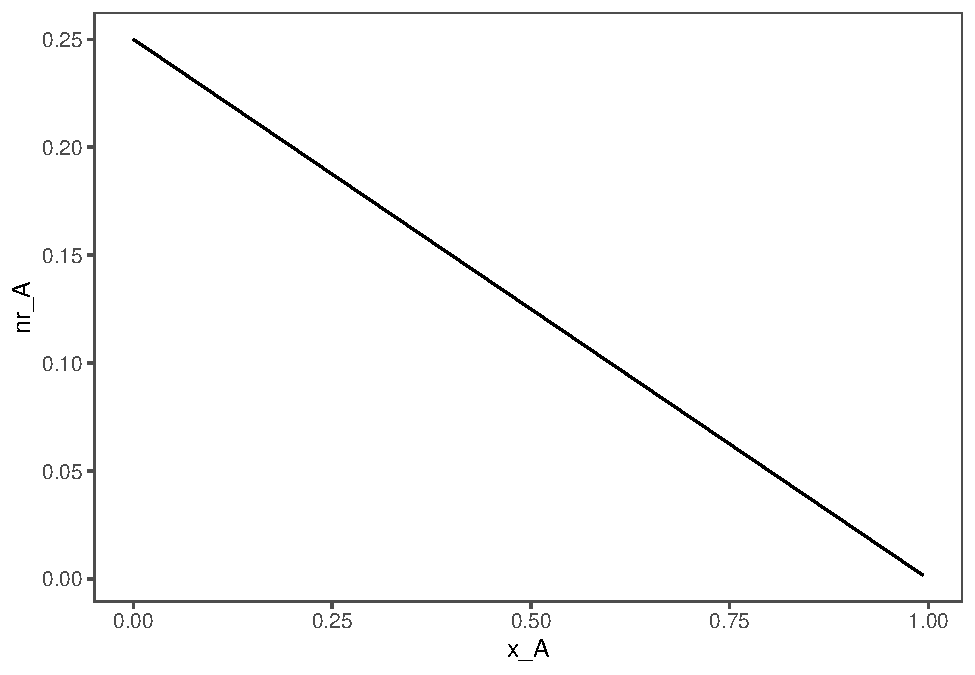
\includegraphics{Bioprocess_Engineering_files/figure-latex/unnamed-chunk-16-1.pdf}

Looking at the PFR equation we can see that instead of a rectangle the \(V/F_{A0}\) ratio is represented by the area under the curve.

\begin{Shaded}
\begin{Highlighting}[]
\FunctionTok{ggplot}\NormalTok{(}\AttributeTok{data =}\NormalTok{ data, }\FunctionTok{aes}\NormalTok{(}\AttributeTok{x =}\NormalTok{ x\_A, }\AttributeTok{y =} \DecValTok{1}\SpecialCharTok{/}\NormalTok{nr\_A)) }\SpecialCharTok{+} \FunctionTok{geom\_line}\NormalTok{() }\SpecialCharTok{+}
    \FunctionTok{annotate}\NormalTok{(}\AttributeTok{geom =} \StringTok{"rect"}\NormalTok{, }\AttributeTok{xmin =} \DecValTok{0}\NormalTok{, }\AttributeTok{xmax =} \FloatTok{0.9}\NormalTok{, }\AttributeTok{ymin =} \DecValTok{0}\NormalTok{,}
        \AttributeTok{ymax =} \DecValTok{1}\SpecialCharTok{/}\NormalTok{data}\SpecialCharTok{$}\NormalTok{nr\_A[}\FunctionTok{min}\NormalTok{(}\FunctionTok{which}\NormalTok{(}\FunctionTok{round}\NormalTok{(data}\SpecialCharTok{$}\NormalTok{x\_A,}
            \DecValTok{3}\NormalTok{) }\SpecialCharTok{==} \FloatTok{0.9}\NormalTok{))], }\AttributeTok{alpha =} \FloatTok{0.5}\NormalTok{) }\SpecialCharTok{+} \FunctionTok{geom\_area}\NormalTok{(}\AttributeTok{mapping =} \FunctionTok{aes}\NormalTok{(}\AttributeTok{x =} \FunctionTok{ifelse}\NormalTok{(x\_A }\SpecialCharTok{\textgreater{}=}
    \DecValTok{0} \SpecialCharTok{\&}\NormalTok{ x\_A }\SpecialCharTok{\textless{}=} \FloatTok{0.9}\NormalTok{, x\_A, }\DecValTok{0}\NormalTok{)), }\AttributeTok{fill =} \StringTok{"red"}\NormalTok{, }\AttributeTok{alpha =} \FloatTok{0.5}\NormalTok{) }\SpecialCharTok{+}
    \FunctionTok{ylim}\NormalTok{(}\FunctionTok{c}\NormalTok{(}\DecValTok{0}\NormalTok{, }\DecValTok{600}\NormalTok{))}
\end{Highlighting}
\end{Shaded}

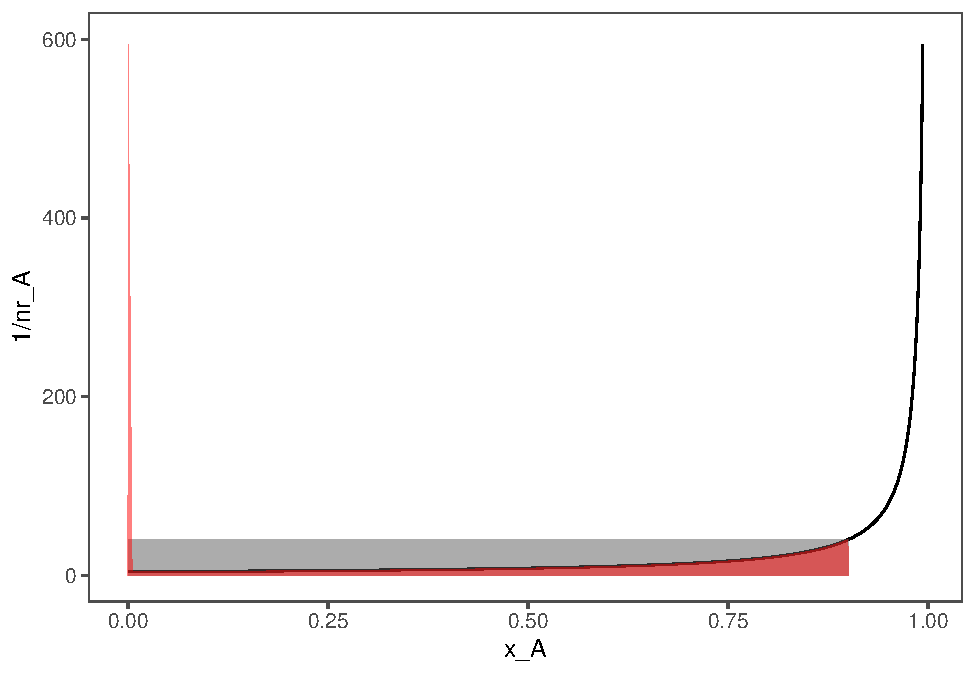
\includegraphics{Bioprocess_Engineering_files/figure-latex/unnamed-chunk-17-1.pdf}

So given a constant flowrate between the two a PFR reactor will be significantly smaller than a CSTR for the same reaction.

\hypertarget{questions-6}{%
\paragraph{???Questions???}\label{questions-6}}

Explain qualitatively why a CSTR needs a larger volume to achieve the same conversion? Hint: what is the average reaction rate in a CSTR vs a PFR?

\begin{quote}
\emph{In a CSTR the reaction rate is always constant as the entire volume is always well mixed. As soon as reactants enter the reactor they are diluted to the effluent conditions, which determine the reaction rate throughout the whole reactor. This dilution does not happen In a PFR, so reactants can enter the reactor at a much higher concentration and therefore the reaction can occur at a much higher initial rate. As the reactants move through the reactor they gradually approach the concentration at which the same reaction would be conducted in a CSTR, finally reaching this concentration as the reach the end of the reactor.}
\end{quote}

\begin{center}\rule{0.5\linewidth}{0.5pt}\end{center}

\hypertarget{kinetics-determining-rate-equations-for-chemical-and-biochemical-reactions}{%
\section{Kinetics: Determining Rate Equations for Chemical and Biochemical Reactions}\label{kinetics-determining-rate-equations-for-chemical-and-biochemical-reactions}}

\hypertarget{remembering-elementary-reactions}{%
\subsection{Remembering Elementary Reactions}\label{remembering-elementary-reactions}}

Remember from Chapter 1 that if a reaction is elementary we can write the rate
of this reaction based on its stoichiometry.

Here, we will make use of this concept to make mathematical models quantifying the kinetics (or reaction rate equations) of complex chemical reactions as well as simple and complex enzymatic reaction. In later chapters we will also apply the ideas developed here to model cells growing in a bioreactor. But before we do that let's discuss some properties of elementary reactions.

What assumptions can we make to help us propose elementary reactions? What are the rules/properties of elementary reactions?

\begin{enumerate}
\def\labelenumi{\arabic{enumi}.}
\item
  An elementary reaction must be simple---a single-step, molecular level event. It likely only involves two molecules, as termolecular collisions are very unlikely, and such collisions happening in the correct orientation are even less likely. We can also assume very few bonds will be formed or broken in a single step.
\item
  Elementary reactions cannot involve fractional molecules.
\item
  Elementary reactions must obey the principle of microscopic reversibility. Microscopic reversibility means that the reaction must follow the same mechanism in the forward and reverse directions. This means that an elementary reaction must be elementary in both directions.
\end{enumerate}

\hypertarget{example-of-an-elementary-reaction}{%
\subsubsection{Example of an elementary reaction}\label{example-of-an-elementary-reaction}}

As an example of an elementary reaction let's consider the decomposition of ozone:
\[ \ce{O3 -> O2 + O^.} \]
In reality, ozone does not decompose spontaneously, ozone collides with dioxygen and the energy of this collision drives decomposition. Thus the reaction written above is not elementary, because it is not written exactly how the reaction happens at the molecular level. We can write the elementary reaction as:
\[ \ce{O3 + O2 -> O2 + O2 + O^.} \]
This equation and that above are both stoichiometrically correct, but the later equation describes the elementary reaction. How do we know this is the elementary reaction? From the rate equation. Fitting experimental data on the decomposition of ozone to the equation for the elementary reaction, \(-r_{O_3} = kC_{O_3}C_{O_2}\), yields a much better fit than \(-r_{O_3} = kC_{O_3}\). We will discuss fitting reaction data to rate equations later on.

\textbf{This iterative process of hypothesizing elementary reactions, based on plausible reaction mechanisms, and fitting experimental data to rate equations derived from these elementary reactions is the basis of chemical and biochemical kinetics.}

With this framework for writing elementary reactions in place we can now begin deriving mechanisms and rate equations for more complex reactions, which are actually series of multiple elementary reactions. Let's look at another more complex example of how a stoichiometrically simple reaction can be broken down into elementary reactions by hypothesizing a mechanism.

\hypertarget{elementary-reactions-provide-feasible-mechanisms}{%
\subsection{Elementary Reactions Provide Feasible Mechanisms}\label{elementary-reactions-provide-feasible-mechanisms}}

Most seemingly simple reactions are not elementary as written but can be broken down into a sequence of elementary reactions. Take for example the Haber-Bosch process, by which most nitrogen for fertilizer is fixed from the atmosphere.
\[ \ce{N2 + 3H2 <=> 2NH3} \]

\hypertarget{questions-7}{%
\paragraph{???Questions???}\label{questions-7}}

How many molecules are involved in the forward and reverse reactions?
How many bonds are formed/broken in the forward and reverse reactions? Is this reaction likely elementary as written? Why or why not?

\begin{quote}
\emph{In the forward reaction 4 species are required to interact simultaneously, which is very unlikely. In the reverse reaction only two species must interact. In the forward reaction 4 bonds must be broken and 6 bonds must be formed, and the opposite is true for the reverse. No, this reaction is not likely elementary as written as the complex interactions and bond rearrangments are highly unlikely in a single step.}
\end{quote}

\begin{center}\rule{0.5\linewidth}{0.5pt}\end{center}

So how does this reaction happen? The Haber-Bosch process relies on a iron catalyst, which facilitates much of this bond breaking and forming by allowing hydrogen and nitrogen species to interact with the catalyst. Let's call the catalyst here \(\ce{S}\) for solid catalyst. \(\ce{S^*}\) will represent a open binding site on the catalyst surface. Now let's write elementary reactions that may constitute a mechanism for the Haber-Bosch process. Initially \(\ce{H2}\) and \(\ce{N2}\) will adsorb onto the catalyst surface.
\[ \ce{H2 + 2S^* <=> 2H-S^*} \]
\[ \ce{N2 + 2S^* <=> 2N-S^*} \]
These forward reactions appear to involve three species, however as our catalyst is solid \(\ce{2S^*}\) act as essentially a single species. Now to form ammonia these adsorbed species must react.
\[ \ce{ N-S^* + H-S^* <=> NH-S^* + S^*} \]
\[ \ce{ NH-S^* + H-S^* <=> NH2-S^* + S^*} \]
\[ \ce{ NH2-S^* + H-S^* <=> NH3-S^* + S^*} \]
And finally the ammonia must desorb from the surface.
\[ \ce{NH3-S^* <=> NH3 + S^*} \]
This proposed mechanism is as simple as possible. The final desorbtion step may happen essentially simultaneously with the final \(\ce{N-H}\) bond formation. We may be able to test this hypothesis with kinetic data or assess under what conditions this assumption might be fair once we have derived a rate equation. But before we derive a rate equation, we should check that the stoichiometry of this series of reactions is equivalent to the complete Haber-Bosch reaction stoichiometry.

We can also write the above balanced chemical reactions as equations in a similar way to how we made a stoichiometric table which can be helpful in dealing with multiple reactions in parallel or series.

\[\sum_i \nu_i A_i = 0\]
where \(A_i\) is each chemical species \(i\) participating in the reaction, and \(\nu_i\) is the stoichiometric coefficient of species \emph{i}.

We can write the above reactions in this form and then sum these equations to determine the net overall reaction.

\[\ce{ - 3H2 - 6S^* + 6H-S^* = 0} \]
\[ \ce{- N2 - 2S^* + 2N-S^* = 0} \]
\[  \ce{ - 2N-S^* - 2H-S^* + 2NH-S^* + 2S^* = 0} \]
\[ \ce{ - 2NH-S^* - 2H-S^* + 2NH2-S^* + 2S^* = 0} \]
\[ \ce{- 2NH2-S^* - 2H-S^* + 2NH3-S^* + 2S^* = 0} \]
\[ \ce{- 2NH3-S^* + 2NH3 + 2S^* = 0} \]
We have to multiply these equations to match the stoichiometry of the overall reaction, but in the end you see that the catalyst sites will cancel out along with the other intermediate species yielding the overall net reaction.
\[\ce{ - N2 - 3H2 + 2NH3 = 0 }\]

Now that we have a mechanism made of elementary reactions that is consistent with the overall reaction, we can write reaction rates for each species in terms of the formation or consumption of that species in each elementary reaction. Then we can solve this set of equations for the rate of the overall reaction in terms of whichever species we'd like, usually the desired product. We won't do that for this very complicated reaction, but will now jump to simple enzyme kinetics as an example.

\hypertarget{summary-kinetics}{%
\subsection{Summary: Kinetics}\label{summary-kinetics}}

Given some non-elementary chemical/biochemical reaction we can define a rate equation for this reaction by the following procedure:

\begin{enumerate}
\def\labelenumi{\arabic{enumi})}
\tightlist
\item
  Define a series of elementary reactions, which are plausible and sum up to the overall reaction. Assign rate constants to each reaction (and direction).
\item
  Write out the differential mass balances for each species in the series of reactions. For each species balance look at each reaction and if that species is being generated or consumed by that elementary reaction, write the appropriate rate for that reaction based on the rule of ``order = stoichiometry'' that applies for elementary reactions.
\item
  You now have a system of differential equations you can use to simulate the reaction!
\item
  To derive a rate equation, pick a species that you want to derive a rate for, typically the product or reactant. Identify the intermediate/unknown/unmeasureable concentrations in the mass balance for that species. You need to replace these with equations derived from the other balances in terms of known quantities.
\item
  Make assumptions to help simplify the system of equations into a single equation (degree of freedom analysis helps here). Is there any step/reaction that might be in equilibrium? What intermediates could you assume to be at steady state? Be sure to note your assumptions and think about when and where they are valid.
\item
  Simplify the the system of equations you have in terms of the intermediates you need to get rid of in your rate equation and plug them in.
\item
  Lump together any combinations of parameters in your equation and define them.
\end{enumerate}

\hypertarget{deriving-enzymatic-rate-equations}{%
\subsection{Deriving enzymatic rate equations}\label{deriving-enzymatic-rate-equations}}

So based on our outlined procedure let's write out some elementary reactions describing how a simple enzyme works. Let's assume an enzyme, \(E\) converts a substrate, \(S\) to product, \(P\):
\[\ce{S ->[E] P}\]
To break this overall reaction up into elementary reactions we need to think about each molecular interaction necessary. First, the enzyme and substrate need to come together in a binding reaction. Then the substrate can be converted to the product in a catalytic step, but still remain bound to the enzyme. Finally the product dissociates from the enzyme. (In the biochemical literature binding and association, and unbinding and dissociation, are used interchangeably). For now all of these reactions could be reversible. So writing out this series as chemical reactions yields the following.
\[\ce{S + E <=>[k_1][k_{-1}] ES}\]
\[\ce{ES <=>[k_2][k_{-2}] EP}\]
\[\ce{EP <=>[k_3][k_{-3}] E + P}\]
In this series of equations we have 5 different species---3 of which we probably can't measure, the active centers \(E\) (free enzyme), \(ES\), and \(EP\)---and 3 independent reactions (reverse reactions are not independent of the forward). We also have 6 unknown parameters, all of the \(k\)'s. So in terms of degrees of freedom this system is solvable for a rate in terms of \(S\) and 4 parameters (these will be combinations of the \emph{k}'s: 6 unknown parameters + 3 unknown variables - 5 equations (one per species) = 4 degrees of freedom. We could write a rate equation for this system if we assume the reactive centers are at steady-state, but the algebra will definitely be tedious. Also, once we get to the final rate equation we may have more parameters than our data can accurately fit. But it is possible to simulate the set of differential equations resulting from this series of reactions relatively easily. We still have many parameters, but we can just give those reasonable and interesting values for demonstration purposes.

So let's write out these equations. We can begin with the general balance for a batch reactor, and write the accumulation term for each species. The for each species balance look at each reaction above and if that species is being generated or consumed by that elementary reaction, write the appropriate rate for that reaction based on the rule of ``order = stoichiometry'' that applies for elementary reactions. Don't forget the reverse reactions!

\[\begin{aligned}
  \text{Accumulation} &= \text{Generation} &-& \text{Consumption}
  \\
  \frac{d[S]}{dt} &= k_{-1}[ES] &-& k_{1}[E][S] 
  \\
  \frac{d[E]}{dt} &= k_{-1}[ES] + k_{3}[EP] &-& k_{1}[E][S] - k_{-3}[E][P] 
  \\
  \frac{d[ES]}{dt} &= k_{1}[E][S] + k_{-2}[EP] &-& k_{-1}[ES] - k_{2}[ES] 
  \\  
  \frac{d[EP]}{dt} &= k_{2}[ES] + k_{-3}[E][P] &-& k_{-2}[EP] - k_{3}[EP] 
  \\
  \frac{d[P]}{dt} &= k_{3}[EP] &-& k_{-3}[E][P] 
\end{aligned}\]

Now to simulate this set of equations we need to define these equations as a differential function.

\begin{Shaded}
\begin{Highlighting}[]
\DocumentationTok{\#\# function defining our differential equations}
\NormalTok{complete\_enzyme\_model }\OtherTok{\textless{}{-}} \ControlFlowTok{function}\NormalTok{(time, curr\_state,}
\NormalTok{    parms) \{}
    \FunctionTok{with}\NormalTok{(}\FunctionTok{as.list}\NormalTok{(}\FunctionTok{c}\NormalTok{(curr\_state, parms)), \{}
        \DocumentationTok{\#\# The with() function gives access to}
        \DocumentationTok{\#\# the named values of parms and}
        \DocumentationTok{\#\# curr\_state within the local function}
        \DocumentationTok{\#\# environment}
\NormalTok{        dSdt }\OtherTok{=}\NormalTok{ k\_n1 }\SpecialCharTok{*}\NormalTok{ ES }\SpecialCharTok{{-}}\NormalTok{ k\_1 }\SpecialCharTok{*}\NormalTok{ E }\SpecialCharTok{*}\NormalTok{ S}
\NormalTok{        dEdt }\OtherTok{=}\NormalTok{ k\_n1 }\SpecialCharTok{*}\NormalTok{ ES }\SpecialCharTok{+}\NormalTok{ k\_3 }\SpecialCharTok{*}\NormalTok{ EP }\SpecialCharTok{{-}}\NormalTok{ k\_1 }\SpecialCharTok{*}\NormalTok{ E }\SpecialCharTok{*}\NormalTok{ S }\SpecialCharTok{{-}}
\NormalTok{            k\_n3 }\SpecialCharTok{*}\NormalTok{ E }\SpecialCharTok{*}\NormalTok{ P}
\NormalTok{        dESdt }\OtherTok{=}\NormalTok{ k\_1 }\SpecialCharTok{*}\NormalTok{ E }\SpecialCharTok{*}\NormalTok{ S }\SpecialCharTok{+}\NormalTok{ k\_n2 }\SpecialCharTok{*}\NormalTok{ EP }\SpecialCharTok{{-}}\NormalTok{ k\_n1 }\SpecialCharTok{*}\NormalTok{ ES }\SpecialCharTok{{-}}
\NormalTok{            k\_2 }\SpecialCharTok{*}\NormalTok{ ES}
\NormalTok{        dEPdt }\OtherTok{=}\NormalTok{ k\_2 }\SpecialCharTok{*}\NormalTok{ ES }\SpecialCharTok{+}\NormalTok{ k\_n3 }\SpecialCharTok{*}\NormalTok{ E }\SpecialCharTok{*}\NormalTok{ P }\SpecialCharTok{{-}}\NormalTok{ k\_n2 }\SpecialCharTok{*}\NormalTok{ EP }\SpecialCharTok{{-}}
\NormalTok{            k\_3 }\SpecialCharTok{*}\NormalTok{ EP}
\NormalTok{        dPdt }\OtherTok{=}\NormalTok{ k\_3 }\SpecialCharTok{*}\NormalTok{ EP }\SpecialCharTok{{-}}\NormalTok{ k\_n3 }\SpecialCharTok{*}\NormalTok{ E }\SpecialCharTok{*}\NormalTok{ P}
        \DocumentationTok{\#\# the computed derivatives are returned}
        \DocumentationTok{\#\# as a list order of derivatives needs}
        \DocumentationTok{\#\# to be the same as the order of species}
        \DocumentationTok{\#\# in curr\_state}
        \FunctionTok{list}\NormalTok{(}\FunctionTok{c}\NormalTok{(dSdt, dEdt, dESdt, dEPdt, dPdt))}
\NormalTok{    \})}
\NormalTok{\}}
\end{Highlighting}
\end{Shaded}

Now we can set the parameter, \(k\) values and initial conditions.

\begin{Shaded}
\begin{Highlighting}[]
\DocumentationTok{\#\# A vector containing the parameter values}
\NormalTok{parms }\OtherTok{\textless{}{-}} \FunctionTok{c}\NormalTok{(}\AttributeTok{k\_1 =} \FloatTok{0.4}\NormalTok{, }\AttributeTok{k\_n1 =} \FloatTok{0.004}\NormalTok{, }\AttributeTok{k\_2 =} \DecValTok{40}\NormalTok{, }\AttributeTok{k\_n2 =} \FloatTok{0.003}\NormalTok{,}
    \AttributeTok{k\_3 =} \DecValTok{1}\NormalTok{, }\AttributeTok{k\_n3 =} \FloatTok{0.003}\NormalTok{)}
\NormalTok{init\_state }\OtherTok{\textless{}{-}} \FunctionTok{c}\NormalTok{(}\AttributeTok{S =} \DecValTok{5}\NormalTok{, }\AttributeTok{E =} \DecValTok{1}\NormalTok{, }\AttributeTok{ES =} \DecValTok{0}\NormalTok{, }\AttributeTok{EP =} \DecValTok{0}\NormalTok{, }\AttributeTok{P =} \DecValTok{0}\NormalTok{)}
\NormalTok{time }\OtherTok{\textless{}{-}} \DecValTok{0}

\FunctionTok{library}\NormalTok{(tidyverse)}
\NormalTok{delta.t }\OtherTok{\textless{}{-}} \FloatTok{0.1}  \DocumentationTok{\#\# 0.1 hours}

\NormalTok{time.out }\OtherTok{\textless{}{-}} \FunctionTok{seq}\NormalTok{(}\DecValTok{0}\NormalTok{, }\DecValTok{20}\NormalTok{, }\AttributeTok{by =}\NormalTok{ delta.t)}

\NormalTok{ts.complete\_enzyme\_model }\OtherTok{\textless{}{-}} \FunctionTok{data.frame}\NormalTok{(deSolve}\SpecialCharTok{::}\FunctionTok{lsoda}\NormalTok{(}\AttributeTok{y =}\NormalTok{ init\_state,}
    \AttributeTok{times =}\NormalTok{ time.out, }\AttributeTok{func =}\NormalTok{ complete\_enzyme\_model,}
    \AttributeTok{parms =}\NormalTok{ parms))}

\NormalTok{ts.complete\_enzyme\_model }\OtherTok{\textless{}{-}}\NormalTok{ tidyr}\SpecialCharTok{::}\FunctionTok{pivot\_longer}\NormalTok{(}\AttributeTok{data =}\NormalTok{ ts.complete\_enzyme\_model,}
    \AttributeTok{cols =} \FunctionTok{c}\NormalTok{(}\StringTok{"S"}\NormalTok{, }\StringTok{"E"}\NormalTok{, }\StringTok{"ES"}\NormalTok{, }\StringTok{"EP"}\NormalTok{, }\StringTok{"P"}\NormalTok{), }\AttributeTok{names\_to =} \StringTok{"Species"}\NormalTok{,}
    \AttributeTok{values\_to =} \StringTok{"Concentration"}\NormalTok{)}

\NormalTok{(complete }\OtherTok{\textless{}{-}} \FunctionTok{ggplot}\NormalTok{(}\AttributeTok{data =}\NormalTok{ ts.complete\_enzyme\_model,}
    \AttributeTok{mapping =} \FunctionTok{aes}\NormalTok{(}\AttributeTok{x =}\NormalTok{ time, }\AttributeTok{y =}\NormalTok{ Concentration, }\AttributeTok{color =}\NormalTok{ Species)) }\SpecialCharTok{+}
    \FunctionTok{geom\_line}\NormalTok{())}
\end{Highlighting}
\end{Shaded}

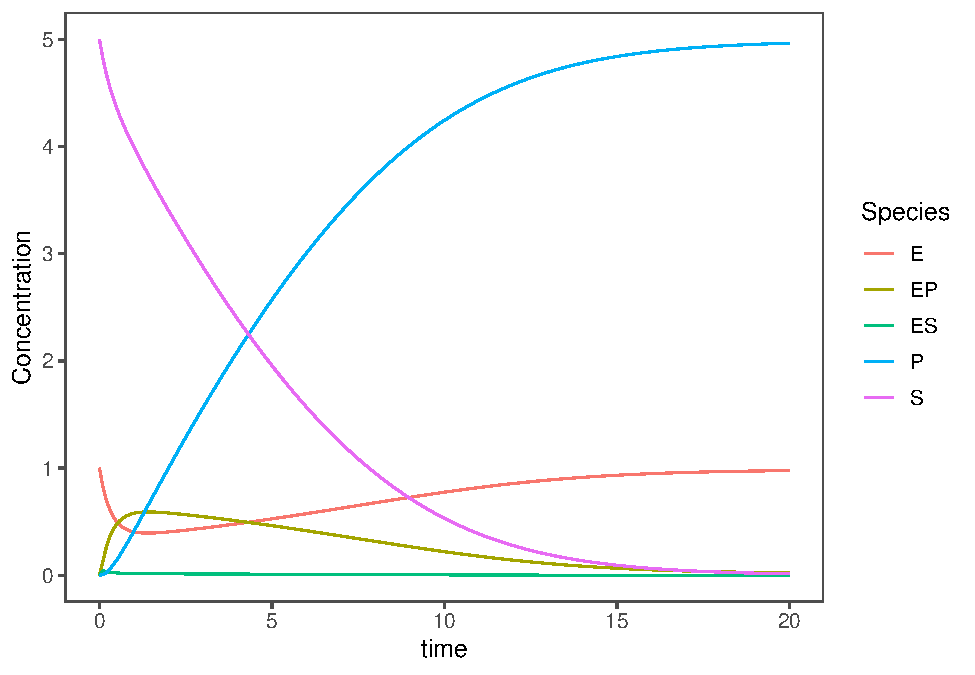
\includegraphics{Bioprocess_Engineering_files/figure-latex/unnamed-chunk-21-1.pdf}

This now gives us a really nice view of each complex and allows us to make some assumptions to simplify our model of enzyme kinetics and check the validity of these assumptions. Bioprocess Engineers and Biochemists typically use a much simpler mechanistic model built on several valid assumptions to describe enzymatic reactions.

To simplify this enzyme reaction mechanism a bit we can make the following assumptions that are likely true for most enzymes:
1) Catalysis is irreversible. This is particularly true in the case inside of cells when products of an enzyme are often further acted upon by other enzymes in a metabolic pathway. It also holds true for the early stages of \emph{in vitro} reactions, when substrate concentrations are high and product concentrations are low. It is also a valid assumption when the \(\Delta G\) of the reaction is large.
2) EP is short lived, enzyme has low affinity for the product. This is generally true for most natural enzymes as in order to bind more substrate and complete another reaction, the product must first be released. So in general enzymes will have much lower binding affinity for their products than their substrates.

\[\ce{S + E <=>[k_1][k_{-1}] ES}\]
\[\ce{ES ->[k_2] E + P}\]

\[\begin{aligned}
  \text{Accumulation} &= \text{Generation} &-& \text{Consumption}
  \\
  \frac{d[S]}{dt} &= k_{-1}[ES] &-& k_{1}[E][S] 
  \\
  \frac{d[E]}{dt} &= k_{-1}[ES] + k_2[ES] &-& k_{1}[E][S]
  \\
  \frac{d[ES]}{dt} &= k_{1}[E][S] &-& k_{-1}[ES] - k_{2}[ES] 
  \\  
  \frac{d[P]}{dt} &= k_{2}[ES]  
\end{aligned}\]

\begin{Shaded}
\begin{Highlighting}[]
\DocumentationTok{\#\# function defining our differential equations}
\NormalTok{simplified\_enzyme\_model }\OtherTok{\textless{}{-}} \ControlFlowTok{function}\NormalTok{(time, curr\_state,}
\NormalTok{    parms) \{}
    \FunctionTok{with}\NormalTok{(}\FunctionTok{as.list}\NormalTok{(}\FunctionTok{c}\NormalTok{(curr\_state, parms)), \{}
        \DocumentationTok{\#\# The with() function gives access to}
        \DocumentationTok{\#\# the named values of parms and}
        \DocumentationTok{\#\# curr\_state within the local function}
        \DocumentationTok{\#\# environment}
\NormalTok{        dSdt }\OtherTok{=}\NormalTok{ k\_n1 }\SpecialCharTok{*}\NormalTok{ ES }\SpecialCharTok{{-}}\NormalTok{ k\_1 }\SpecialCharTok{*}\NormalTok{ E }\SpecialCharTok{*}\NormalTok{ S}
\NormalTok{        dEdt }\OtherTok{=}\NormalTok{ k\_n1 }\SpecialCharTok{*}\NormalTok{ ES }\SpecialCharTok{+}\NormalTok{ k\_2 }\SpecialCharTok{*}\NormalTok{ ES }\SpecialCharTok{{-}}\NormalTok{ k\_1 }\SpecialCharTok{*}\NormalTok{ E }\SpecialCharTok{*}\NormalTok{ S}
\NormalTok{        dESdt }\OtherTok{=}\NormalTok{ k\_1 }\SpecialCharTok{*}\NormalTok{ E }\SpecialCharTok{*}\NormalTok{ S }\SpecialCharTok{{-}}\NormalTok{ k\_1 }\SpecialCharTok{*}\NormalTok{ ES }\SpecialCharTok{{-}}\NormalTok{ k\_2 }\SpecialCharTok{*}\NormalTok{ ES}
\NormalTok{        dPdt }\OtherTok{=}\NormalTok{ k\_2 }\SpecialCharTok{*}\NormalTok{ ES}
        \DocumentationTok{\#\# the computed derivatives are returned}
        \DocumentationTok{\#\# as a list order of derivatives needs}
        \DocumentationTok{\#\# to be the same as the order of species}
        \DocumentationTok{\#\# in curr\_state}
        \FunctionTok{list}\NormalTok{(}\FunctionTok{c}\NormalTok{(dSdt, dEdt, dESdt, dPdt))}
\NormalTok{    \})}
\NormalTok{\}}
\end{Highlighting}
\end{Shaded}

\begin{Shaded}
\begin{Highlighting}[]
\DocumentationTok{\#\# A vector containing the parameter values}
\NormalTok{parms }\OtherTok{\textless{}{-}} \FunctionTok{c}\NormalTok{(}\AttributeTok{k\_1 =} \FloatTok{0.4}\NormalTok{, }\AttributeTok{k\_n1 =} \FloatTok{0.004}\NormalTok{, }\AttributeTok{k\_2 =} \DecValTok{40}\NormalTok{)}
\NormalTok{init\_state }\OtherTok{\textless{}{-}} \FunctionTok{c}\NormalTok{(}\AttributeTok{S =} \DecValTok{5}\NormalTok{, }\AttributeTok{E =} \DecValTok{1}\NormalTok{, }\AttributeTok{ES =} \DecValTok{0}\NormalTok{, }\AttributeTok{P =} \DecValTok{0}\NormalTok{)}
\NormalTok{time }\OtherTok{\textless{}{-}} \DecValTok{0}

\FunctionTok{library}\NormalTok{(tidyverse)}
\NormalTok{delta.t }\OtherTok{\textless{}{-}} \FloatTok{0.1}  \DocumentationTok{\#\# 0.1 hours}

\NormalTok{time.out }\OtherTok{\textless{}{-}} \FunctionTok{seq}\NormalTok{(}\DecValTok{0}\NormalTok{, }\DecValTok{20}\NormalTok{, }\AttributeTok{by =}\NormalTok{ delta.t)}

\NormalTok{ts.simplified\_enzyme\_model }\OtherTok{\textless{}{-}} \FunctionTok{data.frame}\NormalTok{(deSolve}\SpecialCharTok{::}\FunctionTok{lsoda}\NormalTok{(}\AttributeTok{y =}\NormalTok{ init\_state,}
    \AttributeTok{times =}\NormalTok{ time.out, }\AttributeTok{func =}\NormalTok{ simplified\_enzyme\_model,}
    \AttributeTok{parms =}\NormalTok{ parms))}

\NormalTok{ts.simplified\_enzyme\_model }\OtherTok{\textless{}{-}}\NormalTok{ tidyr}\SpecialCharTok{::}\FunctionTok{pivot\_longer}\NormalTok{(}\AttributeTok{data =}\NormalTok{ ts.simplified\_enzyme\_model,}
    \AttributeTok{cols =} \FunctionTok{c}\NormalTok{(}\StringTok{"S"}\NormalTok{, }\StringTok{"E"}\NormalTok{, }\StringTok{"ES"}\NormalTok{, }\StringTok{"P"}\NormalTok{), }\AttributeTok{names\_to =} \StringTok{"Species"}\NormalTok{,}
    \AttributeTok{values\_to =} \StringTok{"Concentration"}\NormalTok{)}

\NormalTok{(simplified }\OtherTok{\textless{}{-}} \FunctionTok{ggplot}\NormalTok{(}\AttributeTok{data =}\NormalTok{ ts.simplified\_enzyme\_model,}
    \AttributeTok{mapping =} \FunctionTok{aes}\NormalTok{(}\AttributeTok{x =}\NormalTok{ time, }\AttributeTok{y =}\NormalTok{ Concentration, }\AttributeTok{color =}\NormalTok{ Species)) }\SpecialCharTok{+}
    \FunctionTok{geom\_line}\NormalTok{())}
\end{Highlighting}
\end{Shaded}

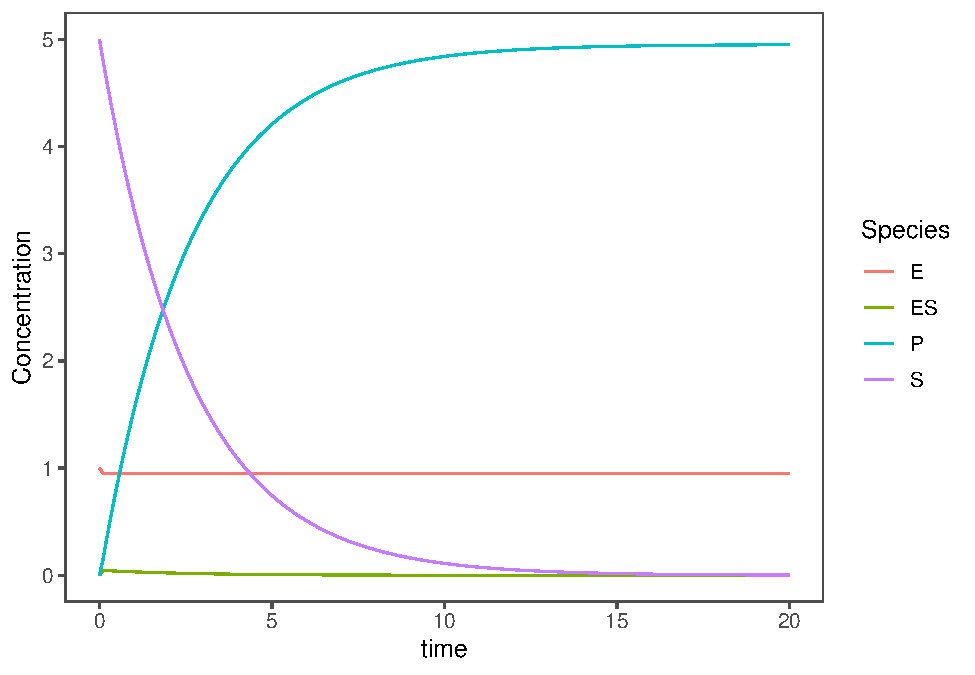
\includegraphics{Bioprocess_Engineering_files/figure-latex/unnamed-chunk-23-1.pdf}

Plotting these next to each other for comparison

\begin{Shaded}
\begin{Highlighting}[]
\FunctionTok{library}\NormalTok{(patchwork)}
\NormalTok{complete }\SpecialCharTok{+}\NormalTok{ simplified}
\end{Highlighting}
\end{Shaded}

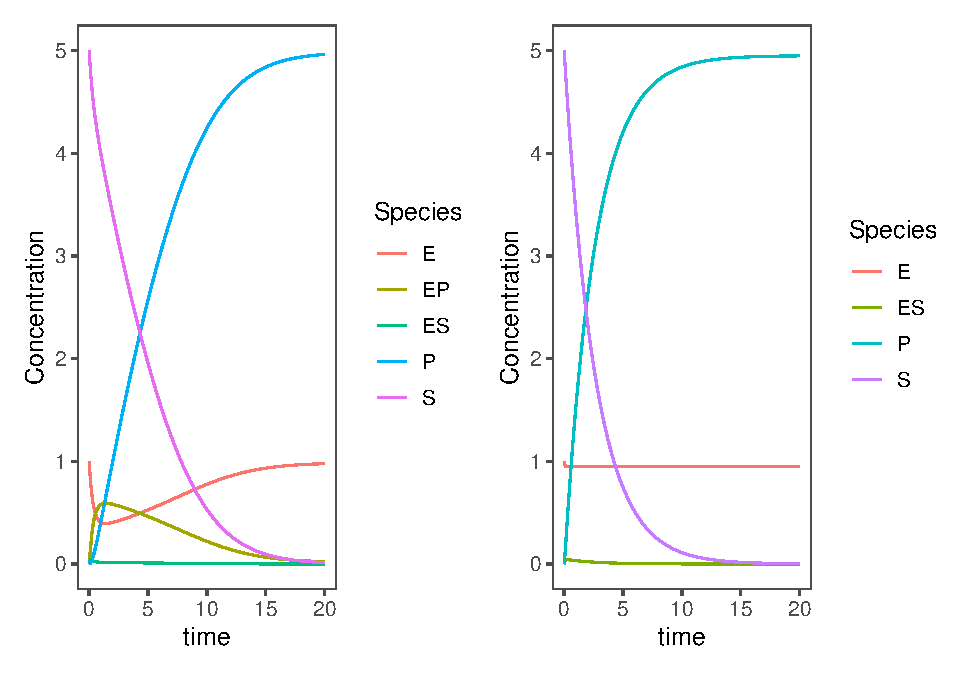
\includegraphics{Bioprocess_Engineering_files/figure-latex/unnamed-chunk-24-1.pdf}

Getting rid of the internal states does, of course, speed up the rate of production of product/consumption of substrate, but we didn't adjust our parameters at all. The \(k_{-2}\), \(k_3\), and \(k_{-3}\) values are all now lumped into \(k_2\) or as it is more typically referred to in this Michaelis-Menten model, \(k_{cat}\). We could change these parameters to better match the original complete model.

\begin{Shaded}
\begin{Highlighting}[]
\DocumentationTok{\#\# A vector containing the parameter values}
\NormalTok{parms }\OtherTok{\textless{}{-}} \FunctionTok{c}\NormalTok{(}\AttributeTok{k\_1 =} \FloatTok{0.3}\NormalTok{, }\AttributeTok{k\_n1 =} \FloatTok{0.004}\NormalTok{, }\AttributeTok{k\_2 =} \DecValTok{5}\NormalTok{)}
\DocumentationTok{\#\# And the initial values and time points}
\NormalTok{init\_state }\OtherTok{\textless{}{-}} \FunctionTok{c}\NormalTok{(}\AttributeTok{S =} \DecValTok{5}\NormalTok{, }\AttributeTok{E =} \DecValTok{1}\NormalTok{, }\AttributeTok{ES =} \DecValTok{0}\NormalTok{, }\AttributeTok{P =} \DecValTok{0}\NormalTok{)}
\NormalTok{time }\OtherTok{\textless{}{-}} \DecValTok{0}
\NormalTok{delta.t }\OtherTok{\textless{}{-}} \FloatTok{0.1}  \DocumentationTok{\#\# 0.1 hours}
\NormalTok{time.out }\OtherTok{\textless{}{-}} \FunctionTok{seq}\NormalTok{(}\DecValTok{0}\NormalTok{, }\DecValTok{20}\NormalTok{, }\AttributeTok{by =}\NormalTok{ delta.t)}

\DocumentationTok{\#\# Now run the model}
\NormalTok{ts.simplified\_enzyme\_model }\OtherTok{\textless{}{-}} \FunctionTok{data.frame}\NormalTok{(deSolve}\SpecialCharTok{::}\FunctionTok{lsoda}\NormalTok{(}\AttributeTok{y =}\NormalTok{ init\_state,}
    \AttributeTok{times =}\NormalTok{ time.out, }\AttributeTok{func =}\NormalTok{ simplified\_enzyme\_model,}
    \AttributeTok{parms =}\NormalTok{ parms))}
\DocumentationTok{\#\# and reformat it for plotting}
\NormalTok{ts.simplified\_enzyme\_model }\OtherTok{\textless{}{-}}\NormalTok{ tidyr}\SpecialCharTok{::}\FunctionTok{pivot\_longer}\NormalTok{(}\AttributeTok{data =}\NormalTok{ ts.simplified\_enzyme\_model,}
    \AttributeTok{cols =} \FunctionTok{c}\NormalTok{(}\StringTok{"S"}\NormalTok{, }\StringTok{"E"}\NormalTok{, }\StringTok{"ES"}\NormalTok{, }\StringTok{"P"}\NormalTok{), }\AttributeTok{names\_to =} \StringTok{"Species"}\NormalTok{,}
    \AttributeTok{values\_to =} \StringTok{"Concentration"}\NormalTok{)}

\DocumentationTok{\#\# and finally plot it}
\NormalTok{simplified }\OtherTok{\textless{}{-}} \FunctionTok{ggplot}\NormalTok{(}\AttributeTok{data =}\NormalTok{ ts.simplified\_enzyme\_model,}
    \AttributeTok{mapping =} \FunctionTok{aes}\NormalTok{(}\AttributeTok{x =}\NormalTok{ time, }\AttributeTok{y =}\NormalTok{ Concentration, }\AttributeTok{color =}\NormalTok{ Species)) }\SpecialCharTok{+}
    \FunctionTok{geom\_line}\NormalTok{()}
\NormalTok{complete }\SpecialCharTok{+}\NormalTok{ simplified}
\end{Highlighting}
\end{Shaded}

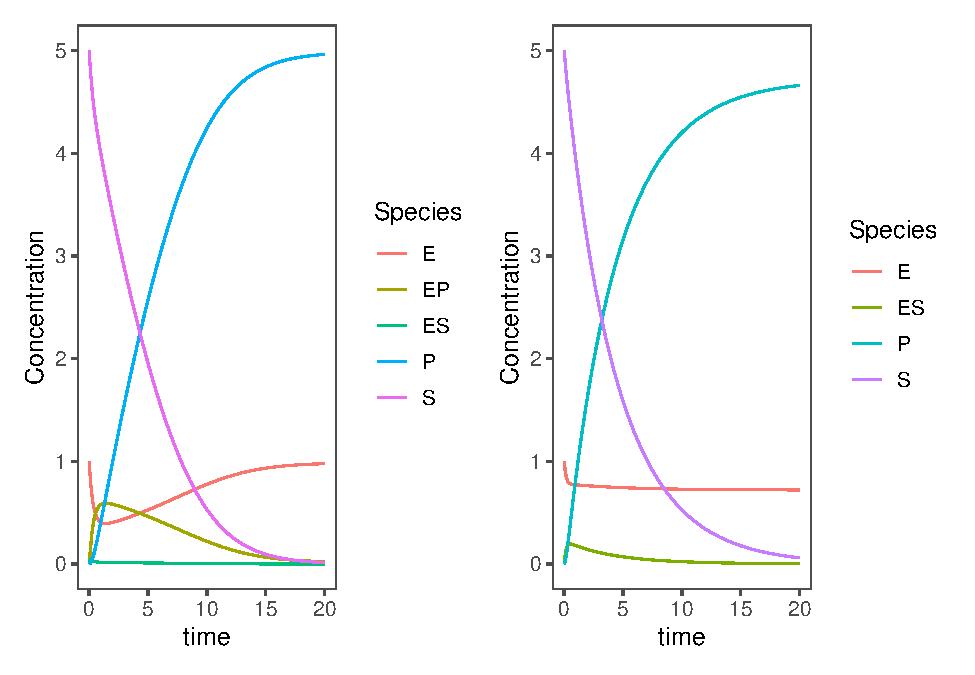
\includegraphics{Bioprocess_Engineering_files/figure-latex/unnamed-chunk-25-1.pdf}

Check out \href{https://stevecheckley.shinyapps.io/shiny_mm/}{this nice shiny app} and play with the sliders to get a feel for what changing each parameter does to the model.

\hypertarget{determining-enzyme-rate-parameters}{%
\section{Determining Enzyme Rate Parameters}\label{determining-enzyme-rate-parameters}}

Now that we have derived plausible rate equations for simple enzymes we need to test how these model equations compare to real experimental reaction rates.

Taking a look at our model:
\[\nu = \frac{V_mS}{K_m + S}\]
where \(V_m = k_{cat}E_0 = k_2E_0\), we find two parameters, \(V_m\) and \(K_m\) which we need to estimate based on experimental data. Although with today's computational power these parameters could be estimated in many possible ways with non-linear regression, historically and still often today linearizations of this enzyme kinetic model are used to fit these parameters to experimental data.

As an aside, we must discuss once again nomenclature issues in the biochemical literature. Unfortunately there is no consensus on what symbol should be used for reaction velocity. In some texts the greek symbol, \(\nu\) (nu), is used in others \(V\), is used. \(V\) can be easily confused with the volume of a reactor, so be sure differentiate your notation when sizing reactors.

\hypertarget{linearization-methods}{%
\subsection{Linearization methods}\label{linearization-methods}}

\hypertarget{lineweaver-burk-plot}{%
\subsubsection{Lineweaver-Burk plot}\label{lineweaver-burk-plot}}

One method of linearization would be to invert the entire model equation.
\[\frac{1}{\nu} = \frac{1}{V_m} + \frac{K_m}{V_m} \frac{1}{S}\]
The resulting plot is called a Lineweaver-Burk plot.

\hypertarget{questions-8}{%
\paragraph{???Questions???}\label{questions-8}}

What would you plot as x and y, and what would be the slope and y-intercept of the plot be.

\begin{quote}
\emph{A Lineweaver-Burke plot is \(1/\nu\) (y) vs \(1/S\) (x). The slope is \(K_m/V_m\) and the y-intercept is \(1/V_m\)}
\end{quote}

\begin{center}\rule{0.5\linewidth}{0.5pt}\end{center}

This plot is also sometimes called a double-reciprocal plot, because we plot the reciprocal of our independent variable \(\nu\) versus our dependent variable \(S\).

To use this plot to find \(V_m\) and \(K_m\) we need to collect reaction velocity data (\(\nu = dP/dt = -dS/dt\)) at different initial substrate concentrations. The reaction velocity will of course decrease throughout the experiment, but to match the initial substrate concentrations, we want to find the initial velocity, i.e.~the initial slope of the curve of product or substrate versus time.

You can perhaps see how determining the instantaneous initial velocity of this curve can be difficult and error prone. We need very rapid and accurate measurements of product or substrate in order to determine this initial slope. Due to the properties of the reciprocal, the error at low substrate concentrations is amplified and has a strong influence on the slope and intercept of the graph. For these reasons the Lineweaver-Burke plot provides better estimates of \(V_m\) than \(K_m\).

\hypertarget{eadie-hofstee-plot}{%
\subsubsection{Eadie-Hofstee Plot}\label{eadie-hofstee-plot}}

To achieve better estimates of \(K_m\) we can use a different linearization and plot of the Michaelis-Menten equation, called the Eadie-Hofstee plot.

\[\nu = V_m - K_m \frac{\nu}{S}\]

In Eadie-Hofstee plot, \(\nu\) is plotted against \(\nu/S\), and \(-K_m\) is the slope and \(V_m\) is the y-intercept. While there is still potential for errors in the calculation of \(\nu\) the issues with low substrate concentrations are lessened. Because the error in \(\nu\) is in x and y coordinates however, this plot does not yield the most accurate measurements of \(V_m\).

\hypertarget{questions-9}{%
\paragraph{???Questions???}\label{questions-9}}

Why does this error not affect the slope?

\begin{quote}
\emph{Error still has the potential to affect the slope, but systematic error will affect both the x and y coordinates equally therefore cancelling the effect of this error on the slope.}
\end{quote}

\begin{center}\rule{0.5\linewidth}{0.5pt}\end{center}

\hypertarget{hanes-woolf-plot}{%
\subsubsection{Hanes-Woolf plot}\label{hanes-woolf-plot}}

There is one more linearization that is commonly used for parameter estimation called the Hanes-Woolf plot. The Hanes-Woolf plot has the form
\[\frac{S}{\nu} = \frac{K_m}{V_m} + \frac{1}{V_m}S\]
Therefore \(S/\nu\) is plotted against \(S\) and \(1/V_m\) is the slope an \(K_m/V_m\) is the y-intercept. The Hanes-Woolf plot accurately estimates \(V_m\), the slope, but again the y-intercept can be innacurate as in this case we cannot measure the reaction velocity at \(S = 0\).

Let's look at an some example data and calculate \(V_m\) and \(K_m\) in several ways. Here we have performed experiments with two different concentrations of the same purified enzyme across a range of substrate concentrations, and calculated the initial velocity of each reaction.

\begin{Shaded}
\begin{Highlighting}[]
\NormalTok{S }\OtherTok{\textless{}{-}} \FunctionTok{c}\NormalTok{(}\DecValTok{20}\NormalTok{, }\DecValTok{10}\NormalTok{, }\FloatTok{6.7}\NormalTok{, }\DecValTok{5}\NormalTok{, }\DecValTok{4}\NormalTok{, }\FloatTok{3.3}\NormalTok{, }\FloatTok{2.9}\NormalTok{, }\FloatTok{2.5}\NormalTok{)  }\CommentTok{\# substrate concentration (g/L)}
\NormalTok{v\_0}\FloatTok{.015} \OtherTok{\textless{}{-}} \FunctionTok{c}\NormalTok{(}\FloatTok{1.14}\NormalTok{, }\FloatTok{0.87}\NormalTok{, }\FloatTok{0.7}\NormalTok{, }\FloatTok{0.59}\NormalTok{, }\FloatTok{0.5}\NormalTok{, }\FloatTok{0.44}\NormalTok{, }\FloatTok{0.39}\NormalTok{,}
    \FloatTok{0.35}\NormalTok{)  }\CommentTok{\# reaction velocity (g/L{-}min) at E\_0 = 0.015 g/L}
\NormalTok{v\_0}\FloatTok{.00875} \OtherTok{\textless{}{-}} \FunctionTok{c}\NormalTok{(}\FloatTok{0.67}\NormalTok{, }\FloatTok{0.51}\NormalTok{, }\FloatTok{0.41}\NormalTok{, }\FloatTok{0.34}\NormalTok{, }\FloatTok{0.29}\NormalTok{, }\ConstantTok{NA}\NormalTok{, }\ConstantTok{NA}\NormalTok{,}
    \ConstantTok{NA}\NormalTok{)  }\CommentTok{\# reaction velocity (g/L{-}min) at E\_0 = 0.00875 g/L}

\NormalTok{data }\OtherTok{\textless{}{-}} \FunctionTok{data.frame}\NormalTok{(S, v\_0}\FloatTok{.015}\NormalTok{, v\_0}\FloatTok{.00875}\NormalTok{)}
\FunctionTok{require}\NormalTok{(knitr)}
\NormalTok{knitr}\SpecialCharTok{::}\FunctionTok{kable}\NormalTok{(data)}
\end{Highlighting}
\end{Shaded}

\begin{tabular}{r|r|r}
\hline
S & v\_0.015 & v\_0.00875\\
\hline
20.0 & 1.14 & 0.67\\
\hline
10.0 & 0.87 & 0.51\\
\hline
6.7 & 0.70 & 0.41\\
\hline
5.0 & 0.59 & 0.34\\
\hline
4.0 & 0.50 & 0.29\\
\hline
3.3 & 0.44 & NA\\
\hline
2.9 & 0.39 & NA\\
\hline
2.5 & 0.35 & NA\\
\hline
\end{tabular}

\begin{quote}
Sometimes we won't know the concentration of our enzyme, if say we are working with just a cell lysate or if we are unable to completly purify our enzyme. In this case we will just use a \emph{specific activity} of the mixture. Specific activity is just the activity of the enzyme per mass of total protein in the complex mixture. The enzyme activity is measure in units of product formed per time at particular conditions (e.g.~temperature, pH, substrate concentration, etc.).
\end{quote}

Let's initially look at this data by plotting \(\nu\) vs \(S\) as dictated by the Michaelis-Menten equation.

\begin{Shaded}
\begin{Highlighting}[]
\FunctionTok{require}\NormalTok{(tidyr)}
\NormalTok{data }\OtherTok{\textless{}{-}}\NormalTok{ tidyr}\SpecialCharTok{::}\FunctionTok{gather}\NormalTok{(}\AttributeTok{data =}\NormalTok{ data, }\AttributeTok{key =}\NormalTok{ E\_0, }\AttributeTok{value =}\NormalTok{ v,}
\NormalTok{    v\_0}\FloatTok{.00875}\NormalTok{, v\_0}\FloatTok{.015}\NormalTok{)}
\FunctionTok{require}\NormalTok{(stringr)}
\NormalTok{data}\SpecialCharTok{$}\NormalTok{E\_0 }\OtherTok{\textless{}{-}} \FunctionTok{as.numeric}\NormalTok{(stringr}\SpecialCharTok{::}\FunctionTok{str\_remove}\NormalTok{(}\AttributeTok{string =}\NormalTok{ data}\SpecialCharTok{$}\NormalTok{E\_0,}
    \AttributeTok{pattern =} \StringTok{"v\_"}\NormalTok{))}
\FunctionTok{require}\NormalTok{(ggplot2)}
\NormalTok{ggplot2}\SpecialCharTok{::}\FunctionTok{ggplot}\NormalTok{(}\AttributeTok{data =}\NormalTok{ data, }\AttributeTok{mapping =} \FunctionTok{aes}\NormalTok{(}\AttributeTok{x =}\NormalTok{ S, }\AttributeTok{y =}\NormalTok{ v,}
    \AttributeTok{color =} \FunctionTok{as.factor}\NormalTok{(E\_0))) }\SpecialCharTok{+} \FunctionTok{geom\_point}\NormalTok{() }\SpecialCharTok{+} \FunctionTok{labs}\NormalTok{(}\AttributeTok{y =} \StringTok{"v (g/L{-}min)"}\NormalTok{,}
    \AttributeTok{x =} \StringTok{"S (g/L)"}\NormalTok{) }\SpecialCharTok{+} \FunctionTok{expand\_limits}\NormalTok{(}\AttributeTok{x =} \DecValTok{0}\NormalTok{, }\AttributeTok{y =} \DecValTok{0}\NormalTok{)}
\end{Highlighting}
\end{Shaded}

\begin{verbatim}
## Warning: Removed 3 rows containing missing values or
## values outside the scale range (`geom_point()`).
\end{verbatim}

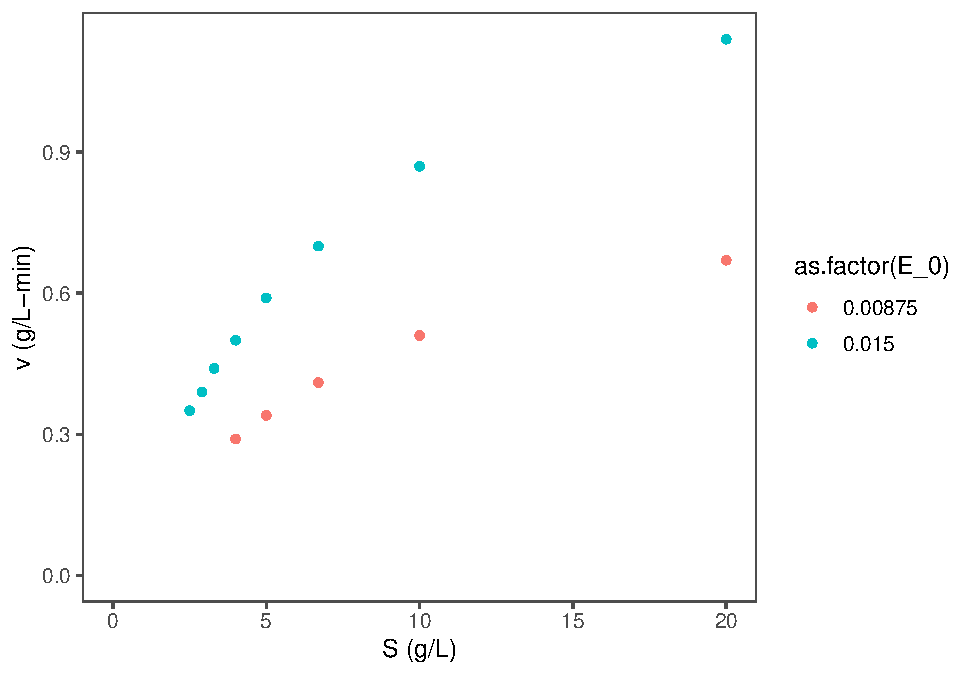
\includegraphics{Bioprocess_Engineering_files/figure-latex/unnamed-chunk-29-1.pdf}

\hypertarget{questions-10}{%
\paragraph{???Questions???}\label{questions-10}}

What can you say about this graph?

\begin{quote}
\emph{The higher concentration of enzyme has a higher velocity across all substrate concentrations. The shape of the two curves is similar. As substrate concentration increases the increase in reaction velocity decreases.}
\end{quote}

\begin{center}\rule{0.5\linewidth}{0.5pt}\end{center}

Now let's make a Lineweaver-Burk plot.
\[\frac{1}{\nu} = \frac{1}{V_m} + \frac{K_m}{V_m} \frac{1}{S}\]

\begin{Shaded}
\begin{Highlighting}[]
\NormalTok{data}\SpecialCharTok{$}\NormalTok{LB.y }\OtherTok{\textless{}{-}} \DecValTok{1}\SpecialCharTok{/}\NormalTok{data}\SpecialCharTok{$}\NormalTok{v}
\NormalTok{data}\SpecialCharTok{$}\NormalTok{LB.x }\OtherTok{\textless{}{-}} \DecValTok{1}\SpecialCharTok{/}\NormalTok{data}\SpecialCharTok{$}\NormalTok{S}
\NormalTok{ggplot2}\SpecialCharTok{::}\FunctionTok{ggplot}\NormalTok{(}\AttributeTok{data =}\NormalTok{ data, }\AttributeTok{mapping =} \FunctionTok{aes}\NormalTok{(}\AttributeTok{x =}\NormalTok{ LB.x,}
    \AttributeTok{y =}\NormalTok{ LB.y, }\AttributeTok{color =} \FunctionTok{as.factor}\NormalTok{(E\_0))) }\SpecialCharTok{+} \FunctionTok{geom\_point}\NormalTok{() }\SpecialCharTok{+}
    \FunctionTok{labs}\NormalTok{(}\AttributeTok{y =} \StringTok{"1/v (L{-}min/g)"}\NormalTok{, }\AttributeTok{x =} \StringTok{"1/S (L/g)"}\NormalTok{) }\SpecialCharTok{+} \FunctionTok{expand\_limits}\NormalTok{(}\AttributeTok{x =} \DecValTok{0}\NormalTok{,}
    \AttributeTok{y =} \DecValTok{0}\NormalTok{)}
\end{Highlighting}
\end{Shaded}

\begin{verbatim}
## Warning: Removed 3 rows containing missing values or
## values outside the scale range (`geom_point()`).
\end{verbatim}

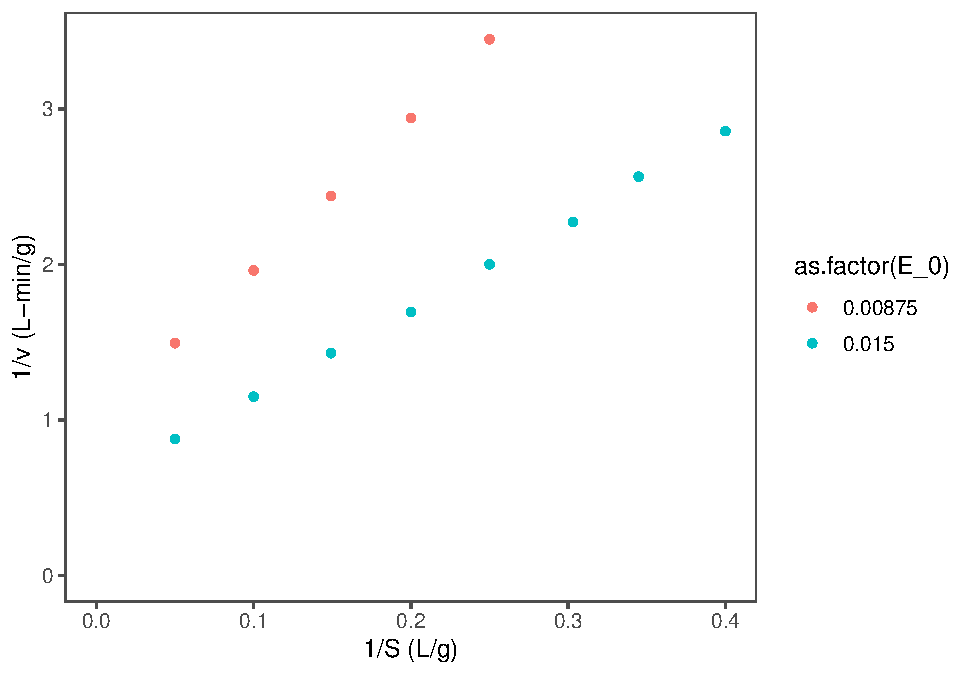
\includegraphics{Bioprocess_Engineering_files/figure-latex/unnamed-chunk-31-1.pdf}

\hypertarget{questions-11}{%
\paragraph{???Questions???}\label{questions-11}}

Why are there two lines here?

\begin{quote}
\emph{Do not forget that \(V_m = k_{cat}E_0\). So the slope of these lines is really \(\frac{K_m}{k_{cat}E_0}\).}
\end{quote}

\begin{center}\rule{0.5\linewidth}{0.5pt}\end{center}

There are two ways that we could go about calculating \(K_m\) and and \(V_m\) or \(k_{cat}\) from this data, either find the slope and intercept of both of the above lines and calcuate 2 parameters and then average them, or we could include the enzyme concentration in our linearization. It is best to do the later as it will allow us to more accurately know the uncertainty in our parameter estimates. To do this we will divide the velocity by \(E_0\) to allow us to linearize the right hand side of the Michaelis-Menten equation in terms of \(k_{cat}\).
\[\nu = \frac{k_{cat}E_0S}{K_m + S}\]
\[\frac{\nu}{E_0} = \frac{k_{cat}S}{K_m + S}\]
Now invert to linearize
\[\frac{E_0}{\nu} = \frac{K_m}{k_{cat}S} + \frac{1}{k_{cat}}\]

So let's now plot \(E_0/\nu\) vs \(1/(S)\).

\begin{Shaded}
\begin{Highlighting}[]
\NormalTok{data}\SpecialCharTok{$}\NormalTok{LB.y }\OtherTok{\textless{}{-}}\NormalTok{ data}\SpecialCharTok{$}\NormalTok{E\_0}\SpecialCharTok{/}\NormalTok{data}\SpecialCharTok{$}\NormalTok{v}
\NormalTok{data}\SpecialCharTok{$}\NormalTok{LB.x }\OtherTok{\textless{}{-}} \DecValTok{1}\SpecialCharTok{/}\NormalTok{data}\SpecialCharTok{$}\NormalTok{S}
\NormalTok{ggplot2}\SpecialCharTok{::}\FunctionTok{ggplot}\NormalTok{(}\AttributeTok{data =}\NormalTok{ data, }\AttributeTok{mapping =} \FunctionTok{aes}\NormalTok{(}\AttributeTok{x =}\NormalTok{ LB.x,}
    \AttributeTok{y =}\NormalTok{ LB.y, }\AttributeTok{color =} \FunctionTok{as.factor}\NormalTok{(E\_0))) }\SpecialCharTok{+} \FunctionTok{geom\_point}\NormalTok{() }\SpecialCharTok{+}
    \FunctionTok{labs}\NormalTok{(}\AttributeTok{y =} \StringTok{"1/v (L{-}min/g)"}\NormalTok{, }\AttributeTok{x =} \StringTok{"1/S (L/g)"}\NormalTok{) }\SpecialCharTok{+} \FunctionTok{expand\_limits}\NormalTok{(}\AttributeTok{x =} \DecValTok{0}\NormalTok{,}
    \AttributeTok{y =} \DecValTok{0}\NormalTok{)}
\end{Highlighting}
\end{Shaded}

\begin{verbatim}
## Warning: Removed 3 rows containing missing values or
## values outside the scale range (`geom_point()`).
\end{verbatim}

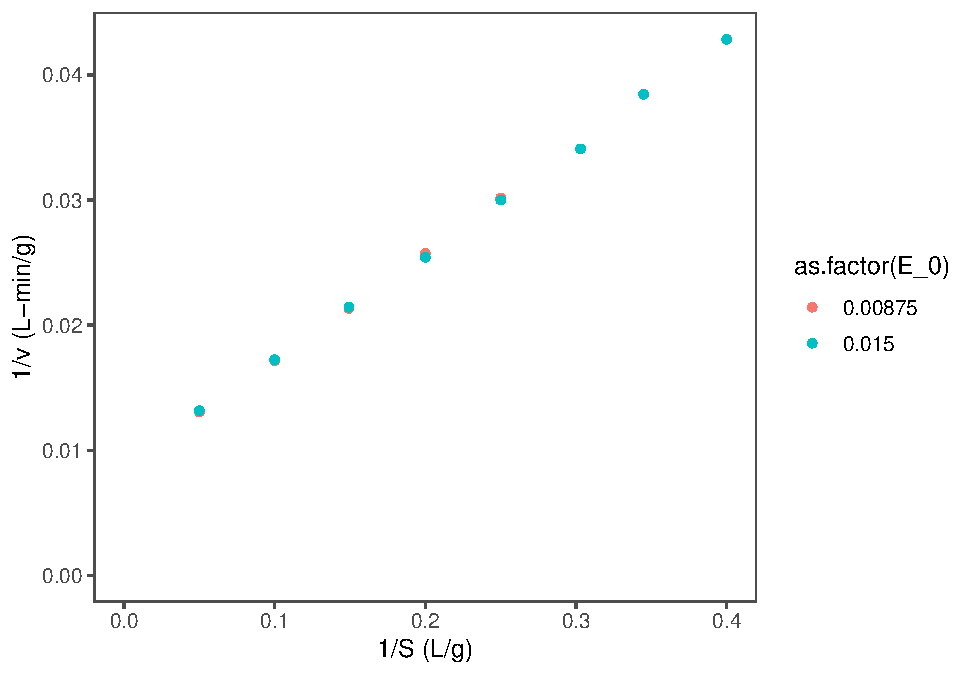
\includegraphics{Bioprocess_Engineering_files/figure-latex/unnamed-chunk-33-1.pdf}

Notice that our two enzyme concentrations now are plotted nearly perfectly overtop of each other. Now we can use linear regression to find the slope and intercept of the line of best fit.

\begin{Shaded}
\begin{Highlighting}[]
\NormalTok{LB }\OtherTok{\textless{}{-}} \FunctionTok{lm}\NormalTok{(}\AttributeTok{formula =}\NormalTok{ LB.y }\SpecialCharTok{\textasciitilde{}}\NormalTok{ LB.x, }\AttributeTok{data =}\NormalTok{ data)}
\FunctionTok{summary}\NormalTok{(LB)}
\end{Highlighting}
\end{Shaded}

\begin{verbatim}
## 
## Call:
## lm(formula = LB.y ~ LB.x, data = data)
## 
## Residuals:
##        Min         1Q     Median         3Q 
## -4.320e-04 -7.006e-05  5.760e-06  9.224e-05 
##        Max 
##  3.779e-04 
## 
## Coefficients:
##              Estimate Std. Error t value Pr(>|t|)
## (Intercept) 0.0087080  0.0001269    68.6 7.84e-16
## LB.x        0.0851892  0.0005698   149.5  < 2e-16
##                
## (Intercept) ***
## LB.x        ***
## ---
## Signif. codes:  
## 0 '***' 0.001 '**' 0.01 '*' 0.05 '.' 0.1 ' ' 1
## 
## Residual standard error: 0.0002181 on 11 degrees of freedom
##   (3 observations deleted due to missingness)
## Multiple R-squared:  0.9995, Adjusted R-squared:  0.9995 
## F-statistic: 2.235e+04 on 1 and 11 DF,  p-value: < 2.2e-16
\end{verbatim}

Looking back at our linearized model,
\[\frac{E_0}{\nu} = \frac{K_m}{k_{cat}S} + \frac{1}{k_{cat}}\]
we can calculate our estimate of \(k_{cat}=\) 114.8369633 \(\pm\) , and our estimate of \(K_m =\) 9.7828737. To calculate the uncertainty in these estimates we must propagate the standard error in our slope and intercept, according to the division formula
\[Q = \frac{a}{x}, \delta Q = Q \sqrt{(\frac{\delta a}{a})^2 + (\frac{\delta x}{x})^2}\]

Let's make a table to compare these estimates with other linearizations as well as nonlinear regression methods.

\begin{Shaded}
\begin{Highlighting}[]
\FunctionTok{require}\NormalTok{(tibble)}
\NormalTok{MM\_params }\OtherTok{\textless{}{-}}\NormalTok{ tibble}\SpecialCharTok{::}\FunctionTok{tibble}\NormalTok{(}\AttributeTok{method =} \StringTok{"LB"}\NormalTok{, }\AttributeTok{k\_cat =} \DecValTok{1}\SpecialCharTok{/}\FunctionTok{summary}\NormalTok{(LB)}\SpecialCharTok{$}\NormalTok{coefficients[}\DecValTok{1}\NormalTok{,}
    \DecValTok{1}\NormalTok{], }\AttributeTok{ek\_cat =} \FunctionTok{summary}\NormalTok{(LB)}\SpecialCharTok{$}\NormalTok{coefficients[}\DecValTok{1}\NormalTok{, }\DecValTok{2}\NormalTok{], }\AttributeTok{K\_m =} \FunctionTok{summary}\NormalTok{(LB)}\SpecialCharTok{$}\NormalTok{coefficients[}\DecValTok{2}\NormalTok{,}
    \DecValTok{1}\NormalTok{]}\SpecialCharTok{/}\FunctionTok{summary}\NormalTok{(LB)}\SpecialCharTok{$}\NormalTok{coefficients[}\DecValTok{1}\NormalTok{, }\DecValTok{1}\NormalTok{], }\AttributeTok{eK\_m =} \FunctionTok{summary}\NormalTok{(LB)}\SpecialCharTok{$}\NormalTok{coefficients[}\DecValTok{2}\NormalTok{,}
    \DecValTok{1}\NormalTok{]}\SpecialCharTok{/}\FunctionTok{summary}\NormalTok{(LB)}\SpecialCharTok{$}\NormalTok{coefficients[}\DecValTok{1}\NormalTok{, }\DecValTok{1}\NormalTok{] }\SpecialCharTok{*} \FunctionTok{sqrt}\NormalTok{((}\FunctionTok{summary}\NormalTok{(LB)}\SpecialCharTok{$}\NormalTok{coefficients[}\DecValTok{1}\NormalTok{,}
    \DecValTok{2}\NormalTok{]}\SpecialCharTok{/}\FunctionTok{summary}\NormalTok{(LB)}\SpecialCharTok{$}\NormalTok{coefficients[}\DecValTok{1}\NormalTok{, }\DecValTok{1}\NormalTok{])}\SpecialCharTok{\^{}}\DecValTok{2} \SpecialCharTok{+}\NormalTok{ (}\FunctionTok{summary}\NormalTok{(LB)}\SpecialCharTok{$}\NormalTok{coefficients[}\DecValTok{2}\NormalTok{,}
    \DecValTok{2}\NormalTok{]}\SpecialCharTok{/}\FunctionTok{summary}\NormalTok{(LB)}\SpecialCharTok{$}\NormalTok{coefficients[}\DecValTok{2}\NormalTok{, }\DecValTok{1}\NormalTok{])}\SpecialCharTok{\^{}}\DecValTok{2}\NormalTok{))}
\NormalTok{knitr}\SpecialCharTok{::}\FunctionTok{kable}\NormalTok{(MM\_params)}
\end{Highlighting}
\end{Shaded}

\begin{tabular}{l|r|r|r|r}
\hline
method & k\_cat & ek\_cat & K\_m & eK\_m\\
\hline
LB & 114.837 & 0.0001269 & 9.782874 & 0.1569057\\
\hline
\end{tabular}

Looking at the linearization for the Eadie-Hofstee plot
\[\nu = V_m - K_m \frac{\nu}{S}\]
We can simplify \(V_m\) to \(k_{cat}E_0\) and then do linear regression as above.

\begin{Shaded}
\begin{Highlighting}[]
\NormalTok{data}\SpecialCharTok{$}\NormalTok{EH.y }\OtherTok{\textless{}{-}}\NormalTok{ data}\SpecialCharTok{$}\NormalTok{v}
\NormalTok{data}\SpecialCharTok{$}\NormalTok{EH.x }\OtherTok{\textless{}{-}}\NormalTok{ data}\SpecialCharTok{$}\NormalTok{v}\SpecialCharTok{/}\NormalTok{data}\SpecialCharTok{$}\NormalTok{S}
\NormalTok{EH }\OtherTok{\textless{}{-}} \FunctionTok{lm}\NormalTok{(}\AttributeTok{formula =}\NormalTok{ EH.y }\SpecialCharTok{\textasciitilde{}}\NormalTok{ E\_0 }\SpecialCharTok{+}\NormalTok{ EH.x }\SpecialCharTok{{-}} \DecValTok{1}\NormalTok{, }\AttributeTok{data =}\NormalTok{ data)}
\FunctionTok{summary}\NormalTok{(EH)}
\end{Highlighting}
\end{Shaded}

\begin{verbatim}
## 
## Call:
## lm(formula = EH.y ~ E_0 + EH.x - 1, data = data)
## 
## Residuals:
##       Min        1Q    Median        3Q       Max 
## -0.022251 -0.007251  0.000530  0.004844  0.020436 
## 
## Coefficients:
##      Estimate Std. Error t value Pr(>|t|)    
## E_0  113.0511     1.0901  103.71  < 2e-16 ***
## EH.x  -9.5441     0.1446  -66.02 1.19e-15 ***
## ---
## Signif. codes:  
## 0 '***' 0.001 '**' 0.01 '*' 0.05 '.' 0.1 ' ' 1
## 
## Residual standard error: 0.01202 on 11 degrees of freedom
##   (3 observations deleted due to missingness)
## Multiple R-squared:  0.9997, Adjusted R-squared:  0.9996 
## F-statistic: 1.623e+04 on 2 and 11 DF,  p-value: < 2.2e-16
\end{verbatim}

\begin{Shaded}
\begin{Highlighting}[]
\NormalTok{MM\_params }\OtherTok{\textless{}{-}} \FunctionTok{rbind}\NormalTok{(MM\_params, }\FunctionTok{c}\NormalTok{(}\StringTok{"EH"}\NormalTok{, }\FunctionTok{summary}\NormalTok{(EH)}\SpecialCharTok{$}\NormalTok{coefficients[[}\DecValTok{1}\NormalTok{,}
    \DecValTok{1}\NormalTok{]], }\FunctionTok{summary}\NormalTok{(EH)}\SpecialCharTok{$}\NormalTok{coefficients[[}\DecValTok{1}\NormalTok{, }\DecValTok{2}\NormalTok{]], }\SpecialCharTok{{-}}\FunctionTok{summary}\NormalTok{(EH)}\SpecialCharTok{$}\NormalTok{coefficients[[}\DecValTok{2}\NormalTok{,}
    \DecValTok{1}\NormalTok{]], }\FunctionTok{summary}\NormalTok{(EH)}\SpecialCharTok{$}\NormalTok{coefficients[[}\DecValTok{2}\NormalTok{, }\DecValTok{2}\NormalTok{]]))}
\NormalTok{knitr}\SpecialCharTok{::}\FunctionTok{kable}\NormalTok{(MM\_params)}
\end{Highlighting}
\end{Shaded}

\begin{tabular}{l|l|l|l|l}
\hline
method & k\_cat & ek\_cat & K\_m & eK\_m\\
\hline
LB & 114.836963256884 & 0.000126942716628018 & 9.78287373281609 & 0.156905735321379\\
\hline
EH & 113.051061858663 & 1.09005061012357 & 9.54408258808163 & 0.144570335085599\\
\hline
\end{tabular}

Now for the Hanes-Woolf plot
\[\frac{S}{\nu} = \frac{K_m}{V_m} + \frac{1}{V_m}S\]

\begin{Shaded}
\begin{Highlighting}[]
\NormalTok{data}\SpecialCharTok{$}\NormalTok{HW.y }\OtherTok{\textless{}{-}}\NormalTok{ data}\SpecialCharTok{$}\NormalTok{E\_0 }\SpecialCharTok{*}\NormalTok{ data}\SpecialCharTok{$}\NormalTok{S}\SpecialCharTok{/}\NormalTok{data}\SpecialCharTok{$}\NormalTok{v}
\NormalTok{HW }\OtherTok{\textless{}{-}} \FunctionTok{lm}\NormalTok{(}\AttributeTok{formula =}\NormalTok{ HW.y }\SpecialCharTok{\textasciitilde{}}\NormalTok{ S, }\AttributeTok{data =}\NormalTok{ data)}
\FunctionTok{summary}\NormalTok{(HW)}
\end{Highlighting}
\end{Shaded}

\begin{verbatim}
## 
## Call:
## lm(formula = HW.y ~ S, data = data)
## 
## Residuals:
##        Min         1Q     Median         3Q 
## -0.0014254 -0.0006425 -0.0000589  0.0007844 
##        Max 
##  0.0016303 
## 
## Coefficients:
##              Estimate Std. Error t value Pr(>|t|)
## (Intercept) 8.417e-02  4.921e-04   171.1   <2e-16
## S           8.874e-03  5.127e-05   173.1   <2e-16
##                
## (Intercept) ***
## S           ***
## ---
## Signif. codes:  
## 0 '***' 0.001 '**' 0.01 '*' 0.05 '.' 0.1 ' ' 1
## 
## Residual standard error: 0.001059 on 11 degrees of freedom
##   (3 observations deleted due to missingness)
## Multiple R-squared:  0.9996, Adjusted R-squared:  0.9996 
## F-statistic: 2.995e+04 on 1 and 11 DF,  p-value: < 2.2e-16
\end{verbatim}

\begin{Shaded}
\begin{Highlighting}[]
\NormalTok{MM\_params }\OtherTok{\textless{}{-}} \FunctionTok{rbind}\NormalTok{(MM\_params, }\FunctionTok{c}\NormalTok{(}\StringTok{"HW"}\NormalTok{, }\DecValTok{1}\SpecialCharTok{/}\FunctionTok{summary}\NormalTok{(HW)}\SpecialCharTok{$}\NormalTok{coefficients[[}\DecValTok{2}\NormalTok{,}
    \DecValTok{1}\NormalTok{]], }\FunctionTok{summary}\NormalTok{(HW)}\SpecialCharTok{$}\NormalTok{coefficients[[}\DecValTok{2}\NormalTok{, }\DecValTok{2}\NormalTok{]], }\FunctionTok{summary}\NormalTok{(HW)}\SpecialCharTok{$}\NormalTok{coefficients[[}\DecValTok{1}\NormalTok{,}
    \DecValTok{1}\NormalTok{]]}\SpecialCharTok{/}\FunctionTok{summary}\NormalTok{(HW)}\SpecialCharTok{$}\NormalTok{coefficients[[}\DecValTok{2}\NormalTok{, }\DecValTok{1}\NormalTok{]], }\FunctionTok{summary}\NormalTok{(HW)}\SpecialCharTok{$}\NormalTok{coefficients[}\DecValTok{2}\NormalTok{,}
    \DecValTok{1}\NormalTok{]}\SpecialCharTok{/}\FunctionTok{summary}\NormalTok{(HW)}\SpecialCharTok{$}\NormalTok{coefficients[}\DecValTok{1}\NormalTok{, }\DecValTok{1}\NormalTok{] }\SpecialCharTok{*} \FunctionTok{sqrt}\NormalTok{((}\FunctionTok{summary}\NormalTok{(HW)}\SpecialCharTok{$}\NormalTok{coefficients[}\DecValTok{1}\NormalTok{,}
    \DecValTok{2}\NormalTok{]}\SpecialCharTok{/}\FunctionTok{summary}\NormalTok{(HW)}\SpecialCharTok{$}\NormalTok{coefficients[}\DecValTok{1}\NormalTok{, }\DecValTok{1}\NormalTok{])}\SpecialCharTok{\^{}}\DecValTok{2} \SpecialCharTok{+}\NormalTok{ (}\FunctionTok{summary}\NormalTok{(HW)}\SpecialCharTok{$}\NormalTok{coefficients[}\DecValTok{2}\NormalTok{,}
    \DecValTok{2}\NormalTok{]}\SpecialCharTok{/}\FunctionTok{summary}\NormalTok{(HW)}\SpecialCharTok{$}\NormalTok{coefficients[}\DecValTok{2}\NormalTok{, }\DecValTok{1}\NormalTok{])}\SpecialCharTok{\^{}}\DecValTok{2}\NormalTok{)))}
\NormalTok{knitr}\SpecialCharTok{::}\FunctionTok{kable}\NormalTok{(MM\_params)}
\end{Highlighting}
\end{Shaded}

\begin{tabular}{l|l|l|l|l}
\hline
method & k\_cat & ek\_cat & K\_m & eK\_m\\
\hline
LB & 114.836963256884 & 0.000126942716628018 & 9.78287373281609 & 0.156905735321379\\
\hline
EH & 113.051061858663 & 1.09005061012357 & 9.54408258808163 & 0.144570335085599\\
\hline
HW & 112.685492138659 & 5.12741049599667e-05 & 9.48505475242782 & 0.000866570502091196\\
\hline
\end{tabular}

\hypertarget{nonlinear-least-squares-regression}{%
\subsection{Nonlinear least squares regression}\label{nonlinear-least-squares-regression}}

With the computational power available today these linearizations are really historical relicts, as we can fit these parameters to our nonlinear model. Nonlinear regression methods essentially sweep through the parameter space, by iteratively changing each parameter and calculating the distance between the model with the current parameter set and the data points. The sum of the squared distance between our model and data is called the residual. The parameter values that minimize the residual are chosen our best fit.

\begin{Shaded}
\begin{Highlighting}[]
\CommentTok{\# Perform nonlinear least squares regression}
\NormalTok{nls1 }\OtherTok{\textless{}{-}} \FunctionTok{nls}\NormalTok{(v }\SpecialCharTok{\textasciitilde{}}\NormalTok{ S}\SpecialCharTok{/}\NormalTok{(S }\SpecialCharTok{+}\NormalTok{ Km) }\SpecialCharTok{*}\NormalTok{ k\_cat }\SpecialCharTok{*}\NormalTok{ E\_0, data, }\FunctionTok{list}\NormalTok{(}\AttributeTok{Km =} \DecValTok{1}\NormalTok{,}
    \AttributeTok{k\_cat =} \DecValTok{1}\NormalTok{))}
\FunctionTok{summary}\NormalTok{(nls1)}
\end{Highlighting}
\end{Shaded}

\begin{verbatim}
## 
## Formula: v ~ S/(S + Km) * k_cat * E_0
## 
## Parameters:
##       Estimate Std. Error t value Pr(>|t|)    
## Km      9.4042     0.1059    88.8   <2e-16 ***
## k_cat 112.1862     0.6591   170.2   <2e-16 ***
## ---
## Signif. codes:  
## 0 '***' 0.001 '**' 0.01 '*' 0.05 '.' 0.1 ' ' 1
## 
## Residual standard error: 0.003881 on 11 degrees of freedom
## 
## Number of iterations to convergence: 11 
## Achieved convergence tolerance: 9.964e-06
##   (3 observations deleted due to missingness)
\end{verbatim}

\begin{Shaded}
\begin{Highlighting}[]
\NormalTok{MM\_params }\OtherTok{\textless{}{-}} \FunctionTok{rbind}\NormalTok{(MM\_params, }\FunctionTok{c}\NormalTok{(}\StringTok{"NLS"}\NormalTok{, }\FunctionTok{summary}\NormalTok{(nls1)}\SpecialCharTok{$}\NormalTok{coefficients[[}\DecValTok{2}\NormalTok{,}
    \DecValTok{1}\NormalTok{]], }\FunctionTok{summary}\NormalTok{(nls1)}\SpecialCharTok{$}\NormalTok{coefficients[[}\DecValTok{2}\NormalTok{, }\DecValTok{2}\NormalTok{]], }\FunctionTok{summary}\NormalTok{(nls1)}\SpecialCharTok{$}\NormalTok{coefficients[[}\DecValTok{1}\NormalTok{,}
    \DecValTok{1}\NormalTok{]], }\FunctionTok{summary}\NormalTok{(nls1)}\SpecialCharTok{$}\NormalTok{coefficients[[}\DecValTok{1}\NormalTok{, }\DecValTok{2}\NormalTok{]]))}
\NormalTok{knitr}\SpecialCharTok{::}\FunctionTok{kable}\NormalTok{(MM\_params)}
\end{Highlighting}
\end{Shaded}

\begin{tabular}{l|l|l|l|l}
\hline
method & k\_cat & ek\_cat & K\_m & eK\_m\\
\hline
LB & 114.836963256884 & 0.000126942716628018 & 9.78287373281609 & 0.156905735321379\\
\hline
EH & 113.051061858663 & 1.09005061012357 & 9.54408258808163 & 0.144570335085599\\
\hline
HW & 112.685492138659 & 5.12741049599667e-05 & 9.48505475242782 & 0.000866570502091196\\
\hline
NLS & 112.18622883779 & 0.659059979310289 & 9.40416797330833 & 0.105901382959763\\
\hline
\end{tabular}

\hypertarget{comparing-linearization-vs-nonlinear-methods}{%
\subsection{Comparing linearization vs nonlinear methods}\label{comparing-linearization-vs-nonlinear-methods}}

The error in each of these parameters is as we expected, based on our knowledge of the linearizations, but which one best fits our actual data? To assess this we can calculate the residuals for each model and compare the sum of the square of these residuals. Let's do this for only the \(E_0 = 0.015\) dataset to keep it simple.

\begin{Shaded}
\begin{Highlighting}[]
\CommentTok{\# Add the correct E\_0 parameter}
\NormalTok{MM\_params}\SpecialCharTok{$}\NormalTok{E\_0 }\OtherTok{\textless{}{-}} \FloatTok{0.015}
\FunctionTok{require}\NormalTok{(tidyverse)}
\CommentTok{\# make sure that the parameters are numerics}
\NormalTok{MM\_params[, }\DecValTok{2}\SpecialCharTok{:}\DecValTok{5}\NormalTok{] }\OtherTok{\textless{}{-}}\NormalTok{ MM\_params[, }\DecValTok{2}\SpecialCharTok{:}\DecValTok{5}\NormalTok{] }\SpecialCharTok{\%\textgreater{}\%}
    \FunctionTok{map}\NormalTok{(as.numeric)}

\CommentTok{\# Write a function to calculate velocity based on}
\CommentTok{\# the Michaelis{-}Menten equation}
\NormalTok{MM }\OtherTok{\textless{}{-}} \ControlFlowTok{function}\NormalTok{(k\_cat, E\_0, S, K\_m) \{}
\NormalTok{    k\_cat }\SpecialCharTok{*}\NormalTok{ E\_0 }\SpecialCharTok{*}\NormalTok{ S}\SpecialCharTok{/}\NormalTok{(K\_m }\SpecialCharTok{+}\NormalTok{ S)}
\NormalTok{\}}

\CommentTok{\# Write a for loop to calculate velocity for each}
\CommentTok{\# S value with each parameter set}
\NormalTok{resid }\OtherTok{\textless{}{-}} \FunctionTok{tibble}\NormalTok{(S, v\_0}\FloatTok{.015}\NormalTok{)}
\ControlFlowTok{for}\NormalTok{ (i }\ControlFlowTok{in} \DecValTok{1}\SpecialCharTok{:}\FunctionTok{nrow}\NormalTok{(MM\_params)) \{}
    \CommentTok{\# calculate predicted v values}
\NormalTok{    v }\OtherTok{\textless{}{-}} \FunctionTok{with}\NormalTok{(MM\_params[i, ], \{}
        \FunctionTok{MM}\NormalTok{(k\_cat, E\_0, S, K\_m)}
\NormalTok{    \})}
    \CommentTok{\# name the predicted column with the method}
    \CommentTok{\# and add it to resid}
\NormalTok{    resid }\OtherTok{\textless{}{-}}\NormalTok{ resid }\SpecialCharTok{\%\textgreater{}\%}
        \FunctionTok{add\_column}\NormalTok{(}\SpecialCharTok{!!}\NormalTok{(MM\_params[[i, }\StringTok{"method"}\NormalTok{]]) }\SpecialCharTok{:=}
\NormalTok{            v)}
\NormalTok{\}}
\NormalTok{resid}
\end{Highlighting}
\end{Shaded}

\begin{verbatim}
## # A tibble: 8 x 6
##       S v_0.015    LB    EH    HW   NLS
##   <dbl>   <dbl> <dbl> <dbl> <dbl> <dbl>
## 1  20      1.14 1.16  1.15  1.15  1.14 
## 2  10      0.87 0.871 0.868 0.867 0.867
## 3   6.7    0.7  0.700 0.699 0.700 0.700
## 4   5      0.59 0.583 0.583 0.583 0.584
## 5   4      0.5  0.500 0.501 0.501 0.502
## 6   3.3    0.44 0.434 0.436 0.436 0.437
## 7   2.9    0.39 0.394 0.395 0.396 0.397
## 8   2.5    0.35 0.351 0.352 0.353 0.353
\end{verbatim}

\begin{Shaded}
\begin{Highlighting}[]
\CommentTok{\# Calculate the residuals for each method}
\NormalTok{resid }\OtherTok{\textless{}{-}}\NormalTok{ resid }\SpecialCharTok{\%\textgreater{}\%}
    \FunctionTok{mutate\_at}\NormalTok{(}\FunctionTok{c}\NormalTok{(}\StringTok{"LB"}\NormalTok{, }\StringTok{"EH"}\NormalTok{, }\StringTok{"HW"}\NormalTok{, }\StringTok{"NLS"}\NormalTok{), }\AttributeTok{.funs =} \FunctionTok{funs}\NormalTok{(. }\SpecialCharTok{{-}}
\NormalTok{        v\_0}\FloatTok{.015}\NormalTok{))  }\CommentTok{\# . = predicted}
\end{Highlighting}
\end{Shaded}

\begin{verbatim}
## Warning: `funs()` was deprecated in dplyr 0.8.0.
## i Please use a list of either functions or
##   lambdas:
## 
## # Simple named list: list(mean = mean, median =
##   median)
## 
## # Auto named with `tibble::lst()`:
##   tibble::lst(mean, median)
## 
## # Using lambdas list(~ mean(., trim = .2), ~
##   median(., na.rm = TRUE))
## Call `lifecycle::last_lifecycle_warnings()` to
## see where this warning was generated.
\end{verbatim}

\begin{Shaded}
\begin{Highlighting}[]
\CommentTok{\# Calculate the sum of the square of residuals}
\NormalTok{SSR }\OtherTok{\textless{}{-}}\NormalTok{ resid }\SpecialCharTok{\%\textgreater{}\%}
    \FunctionTok{summarise\_at}\NormalTok{(}\FunctionTok{c}\NormalTok{(}\StringTok{"LB"}\NormalTok{, }\StringTok{"EH"}\NormalTok{, }\StringTok{"HW"}\NormalTok{, }\StringTok{"NLS"}\NormalTok{), }\AttributeTok{.funs =} \FunctionTok{funs}\NormalTok{(}\FunctionTok{sum}\NormalTok{(.}\SpecialCharTok{\^{}}\DecValTok{2}\NormalTok{)))}
\end{Highlighting}
\end{Shaded}

\begin{verbatim}
## Warning: `funs()` was deprecated in dplyr 0.8.0.
## i Please use a list of either functions or
##   lambdas:
## 
## # Simple named list: list(mean = mean, median =
##   median)
## 
## # Auto named with `tibble::lst()`:
##   tibble::lst(mean, median)
## 
## # Using lambdas list(~ mean(., trim = .2), ~
##   median(., na.rm = TRUE))
## Call `lifecycle::last_lifecycle_warnings()` to
## see where this warning was generated.
\end{verbatim}

\begin{Shaded}
\begin{Highlighting}[]
\CommentTok{\# Plot the SSR values}
\NormalTok{SSR }\OtherTok{\textless{}{-}} \FunctionTok{gather}\NormalTok{(SSR, }\AttributeTok{key =} \StringTok{"method"}\NormalTok{, }\AttributeTok{value =} \StringTok{"SSR"}\NormalTok{)}
\FunctionTok{ggplot}\NormalTok{(}\AttributeTok{data =}\NormalTok{ SSR, }\AttributeTok{mapping =} \FunctionTok{aes}\NormalTok{(}\AttributeTok{x =}\NormalTok{ forcats}\SpecialCharTok{::}\FunctionTok{fct\_inorder}\NormalTok{(method),}
    \AttributeTok{y =}\NormalTok{ SSR)) }\SpecialCharTok{+} \FunctionTok{geom\_bar}\NormalTok{(}\AttributeTok{stat =} \StringTok{"identity"}\NormalTok{) }\SpecialCharTok{+} \FunctionTok{labs}\NormalTok{(}\AttributeTok{x =} \StringTok{"method"}\NormalTok{,}
    \AttributeTok{y =} \StringTok{"Sum of square residuals"}\NormalTok{)}
\end{Highlighting}
\end{Shaded}

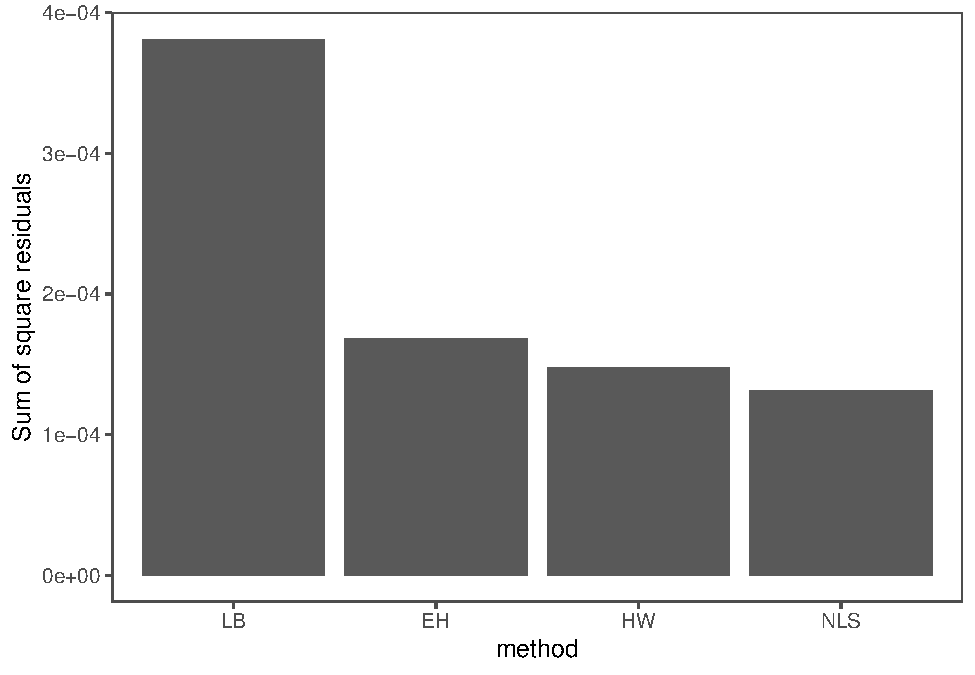
\includegraphics{Bioprocess_Engineering_files/figure-latex/unnamed-chunk-39-1.pdf}

So you can see in this case that the nonlinear least squares regression results in the best fit. In general this will be the case. We could also combine the \(K_m\) from Eadie-Hofstee and the \(V_m\) from Hanes-Woolf, but we still run into the issue of these linear transformations skewing our uncertainty in or parameters. Nonlinear regression methods yield absolute uncertainties in the parameter estimates that can be easily compared and interpreted.

Just for fun let's see what the difference in these models looks like.

\begin{Shaded}
\begin{Highlighting}[]
\NormalTok{S\_plot }\OtherTok{\textless{}{-}} \FunctionTok{seq}\NormalTok{(}\DecValTok{0}\NormalTok{, }\DecValTok{25}\NormalTok{, }\FloatTok{0.1}\NormalTok{)}
\NormalTok{model\_plot }\OtherTok{\textless{}{-}} \FunctionTok{tibble}\NormalTok{(S\_plot)}
\ControlFlowTok{for}\NormalTok{ (i }\ControlFlowTok{in} \DecValTok{1}\SpecialCharTok{:}\FunctionTok{nrow}\NormalTok{(MM\_params)) \{}
    \CommentTok{\# calculate predicted v values}
\NormalTok{    v }\OtherTok{\textless{}{-}} \FunctionTok{with}\NormalTok{(MM\_params[i, ], \{}
        \FunctionTok{MM}\NormalTok{(k\_cat, E\_0, S\_plot, K\_m)}
\NormalTok{    \})}
    \CommentTok{\# name the predicted column with the method}
    \CommentTok{\# and add it to resid}
\NormalTok{    model\_plot }\OtherTok{\textless{}{-}}\NormalTok{ model\_plot }\SpecialCharTok{\%\textgreater{}\%}
        \FunctionTok{add\_column}\NormalTok{(}\SpecialCharTok{!!}\NormalTok{(MM\_params[[i, }\StringTok{"method"}\NormalTok{]]) }\SpecialCharTok{:=}
\NormalTok{            v)}
\NormalTok{\}}

\NormalTok{model\_plot }\OtherTok{\textless{}{-}}\NormalTok{ model\_plot }\SpecialCharTok{\%\textgreater{}\%}
    \FunctionTok{gather}\NormalTok{(}\AttributeTok{key =} \StringTok{"method"}\NormalTok{, }\AttributeTok{value =} \StringTok{"v"}\NormalTok{, }\DecValTok{2}\SpecialCharTok{:}\DecValTok{5}\NormalTok{)}

\FunctionTok{ggplot}\NormalTok{(}\AttributeTok{data =}\NormalTok{ model\_plot, }\AttributeTok{mapping =} \FunctionTok{aes}\NormalTok{(}\AttributeTok{x =}\NormalTok{ S\_plot,}
    \AttributeTok{y =}\NormalTok{ v, }\AttributeTok{color =}\NormalTok{ method)) }\SpecialCharTok{+} \FunctionTok{geom\_line}\NormalTok{() }\SpecialCharTok{+} \FunctionTok{labs}\NormalTok{(}\AttributeTok{x =} \StringTok{"Velocity g/L{-}min"}\NormalTok{,}
    \AttributeTok{y =} \StringTok{"Substrate g/L"}\NormalTok{)}
\end{Highlighting}
\end{Shaded}

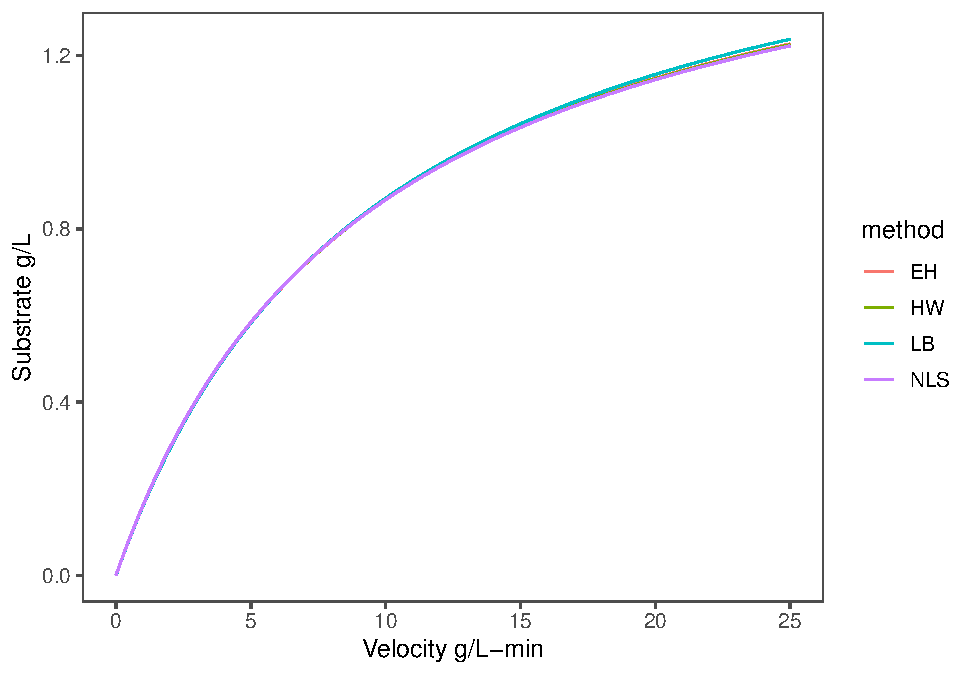
\includegraphics{Bioprocess_Engineering_files/figure-latex/unnamed-chunk-40-1.pdf}

\href{https://drclongstaff.shinyapps.io/MichaelisMentenCL/}{This is a decent shiny app for demonstrating parameter fitting.}

\href{https://sites.duke.edu/bossbackup/files/2013/02/nonlime.pdf}{Here is a demonstration of linear and nonlinear fitting with MATLAB.}

\hypertarget{complex-enzyme-kinetics}{%
\section{Complex Enzyme Kinetics}\label{complex-enzyme-kinetics}}

Many enzymes do not simply convert one substrate to a single product. Enzymes such as amylases which are critical to brewing and distilling convert long chains of sugars (starches) into shorter chains and disaccharides.

\hypertarget{allosteric-enzymes}{%
\subsection{Allosteric Enzymes}\label{allosteric-enzymes}}

Allosteric enzymes have more than one substrate binding site, or an ``effector'' binding site in addition to a substrate binding site. An effector can be any biomolecule, that when bound to the enzyme, affects the activity of the enzyme.

If the effector or substrate has a positive effect on enzyme activity this is called cooperativity.

\hypertarget{enzyme-inhibition}{%
\subsection{Enzyme Inhibition}\label{enzyme-inhibition}}

\hypertarget{competitive-inhibition}{%
\subsubsection{Competitive Inhibition}\label{competitive-inhibition}}

\hypertarget{uncompetitive}{%
\subsubsection{Uncompetitive}\label{uncompetitive}}

\hypertarget{noncompetitive}{%
\subsubsection{Noncompetitive}\label{noncompetitive}}

\hypertarget{substrate-inhibition}{%
\subsubsection{Substrate Inhibition}\label{substrate-inhibition}}

\end{document}
